\documentclass{tstextbook}

\begin{document}

\tsbook{Projet Tatamis}
       {ANGER Benoit - BOURGINE Bruno}
       {Utagawa Hiroshige / Carrie May}
       {2021-2022}
       {xxxxx}{xxx--xx--xxxx--xx--x}{0.1}
       {}
       {}

%---------------------------------------------------------------------------
% Chapters
%---------------------------------------------------------------------------

%---------------------------------------------------------------------------

\chapter{Présentation}
\begin{summary}
    Ce premier chapitre sera l'occasion d'introduire le projet tel qu'il a été initié et de 
    détailler les outils et les méthodes envisagées pour son développement.
  \end{summary}

\section{Descriptif de la problématique}


Le pavage du plan avec des rectangle est un problème classique et déjà largement documenté,
mais je souhaite l'aborder par un aspect très concret : étant donné un nombre de tatamis, quelles sont les
configurations possibles.\\
\begin{center}
    \includegraphics[width = 0.5\linewidth]{./images/pavage-par-tatamis.png}
\end{center}
C'est un problème que rencontre notamment toute personne qui se retrouve à devoir installer un dojo.
Il existe une contrainte de base qui est que 4 tatamis ne rejoignent jamais en un même coin. Mais ont peut
en ajouter d'autres : possibilité de demi-tatamis (carré), répartition des couleurs, répartition de l'usure...

\section{Ébauche de cahier des charges}

Utilisateur final : gestionnaire de dojo\\

L'interface utilisateur devra comprendre un menu de paramétrage basique : nombre de tatamis,
contraintes géométriques, contraintes d'aspect général; ainsi qu'un affichage des dispositions envisageables.\\

L'utilisateur devra pouvoir saisir :

\begin{itemize}
    \item le nombre et le type (entier/demis) de tatamis à disposition
    \item leurs dimensions
    \item leurs couleurs
    \item éventuellement leur état (on dispose de préférence les plus usés en périphérie)
    \item les dimensions du dojo
\end{itemize}

L'affichage proposera différentes disposition selon les contraintes imposées.

\section{Membres du projet}

\begin{itemize}
    \item ANGER Benoit, étudiant licence L3 MATH-Infos
    \item BOURGINE Bruno, étudiant DU CCIE
    \item BOULALEH Ismail, étudiant licence L3 MATH-Infos (prévu initialement, mais n'a finalement pas
    participé au projet)
\end{itemize}



\chapter{Cahier des charges}
\section{Démarche}

La problématique initiale telle qu'elle a été énoncée est la suivante : \emph{étant donné un nombre de tatamis, quelles sont les 
configurations possibles ?}\\

Les dojos sont de dimension m (hauteur) x n (largeur) unités. Et les tatamis sont de dimension 1 x 2 unités. Il existe parfois des demi-tatamis de dimension 1 x 1 unité.
Pour disposer les tatamis, il existe une contrainte: quatre coins de tatamis ne peuvent pas se retrouver en un même point.

Nous allons ici détaillé plus précisément le cahier des charges de l'application. Nous listerons les \emph{epics} afin d'en déduire
les \emph{users stories} et leurs tâches afférentes, et ainsi établir la \emph{roadmap} de notre projet. Le cahier des charges est formulé 
du point de vue de l'utilisateur final, les \emph{epics} étant rédigées sous la forme : \emph{en tant que} \dots ,\emph{je souhaite} \dots ,\emph{afin de } \dots.\\


Par ailleurs afin de prioriser les demandes, nous classerons les fonctionnalités en deux catégories :

\begin{itemize}
    \item essentielles (must have)
    \item optionnelles (nice to have)
\end{itemize}

\section{Persona de l’utilisateur final}

L’utilisateur final est un gestionnaire de dojo.\\

A propos:
\begin{itemize}
    \item Les gestionnaires de dojo ont des profils et backgrounds variés. Il peut être très avancé 
    ou très novice en informatique et en géométrie
    \item En revanche, avec un peu de formation et si on lui installe les outils, il sera capable 
    des les utiliser même si l’ergonomie n’est pas idéale
\end{itemize}


Objectifs:
\begin{itemize}
    \item Préparer le dojo pour qu’il soit prêt pour les entraînements et compétitions
    \item Assurer l’usure équitable des tatamis par des modifications régulières de disposition
\end{itemize}

Points de douleur:
\begin{itemize}
    \item Quand il arrive sur un nouveau dojo, il est difficile de savoir rapidement si une 
    combinaison de tatami est possible ou non
    \item Il est également difficile de savoir combien de tatamis lui sont nécessaires pour 
    faire le dojo
    \item A chaque fois qu’il faut nettoyer le dojo, il faut enlever tous les tatamis, et 
    il est compliqué de refaire le dojo
    \item En particulier lorsqu’il a des demi-tatamis ou des tatamis de couleurs différentes

\end{itemize}



\section{Fonctionnalités essentielles}

%\item \emph{En tant que } gestionnaire de dojo,\emph{ je souhaite} ... \emph{ afin de }...

\begin{itemize}
    \item En tant que gestionnaire de dojo, je souhaite savoir s’il existe une solution pour
     un dojo d'une dimension donnée, afin de savoir si je pourrais remplir mon dojo ou non.
\end{itemize}


\textbf{ Si une solution existe :}

\begin{itemize}
    \item \emph{En tant que} gestionnaire de dojo, 
    \emph{ je souhaite} connaître le nombre de tatamis nécessaires pour un dojo d'une dimension donnée,
    \emph{afin de } n’en déployer que le nombre nécessaire.
    \item \emph{En tant que} gestionnaire de dojo,
    \emph{ je souhaite} connaître le nombre de dispositions possibles pour un dojo d'une dimension donnée, 
    \emph{ afin d'}anticiper la complexité du placement des tatamis.
    \item \emph{En tant que} gestionnaire de dojo ,
    \emph{ je souhaite} visualiser l'ensemble des dispositions possibles, pour un dojo d'une dimension donnée
    \emph{afin de } m’aider à placer les tatamis sur mon dojo.
    \item \emph{En tant que} gestionnaire de dojo, 
    \emph{ je souhaite} pouvoir renseigner le nombre de tatamis dont je dispose, 
    \emph{afin d'}obtenir une solution adaptée à mon matériel.
    \item \emph{En tant que} gestionnaire de dojo,
    \emph{ je souhaite} voir afficher les dimensions (longueur, largeur, surface) des dispositions proposées  
    \emph{ afin d' }exploiter aux mieux l'espace disponible à l'intérieur et à l'extérieur du tatamis.
\end{itemize}


\section{Fonctionnalités optionnelles}


\begin{itemize}
    \item \emph{En tant que} gestionnaire de dojo, 
    \emph{ je souhaite} connaître le nombre de dispositions possibles, modulo une rotation ou une symétrie 
    \emph{ afin de } ne voir sur l’écran que les solutions réellement différentes.
    \item \emph{En tant que} gestionnaire de dojo, 
    \emph{ je souhaite} visualiser l’ensemble des dispositions possibles, modulo une rotation ou une symétrie 
    \emph{ afin de } ne voir sur l’écran que les solutions réellement différentes.
    % \item \emph{En tant que } gestionnaire de dojo,
    % \emph{ je souhaite} je souhaite savoir s'il est utile d’utiliser des demi-tatamis
    % \emph{ afin de } trouver une solution quand elle n’existe pas sans demi-tatamis.
    % \item \emph{En tant que } gestionnaire de dojo,
    % \emph{ je souhaite} avoir visuellement les dispositions possibles en utilisant un nombre donné de demi-tatamis
    % \emph{ afin de } pouvoir exploiter tous les demi-tatamis dont je dispose. 
    \item \emph{En tant que } gestionnaire de dojo,
    \emph{ je souhaite} pouvoir modifier les dimensions d'un tatamis
     \emph{ afin de } obtenir des propositions correspondant à mon matériel.
    \item \emph{En tant que } gestionnaire de dojo,
    \emph{ je souhaite} pouvoir créer des catégories de couleurs de tatamis
     \emph{ afin de } visualiser des propositions de placement avec les couleurs réelles.
    % \item \emph{En tant que } gestionnaire de dojo,
    % \emph{ je souhaite} pouvoir renseigner des critères de placement (par exemple une symétrie, un motif particulier…) 
    % \emph{ afin de } disposer de la meilleure solution selon moi.
\end{itemize}

\chapter{Méthodologie}
\section{Choix de méthodologie}

La méthodologie agile nous paraît très adaptée au développement de notre programme.
En effet, la méthodologie agile:

\begin{itemize}
    \item  Est particulièrement adaptée à la résolution de problèmes complexes
          à solutions incertaines ou l’on ne sait pas forcément avec précisions l’objectif
          final ou la manière d’y arriver, ce qui est notre cas
    \item Est basée sur l'itération avec la production de livrables testables
          à la fin de chaque \emph{sprint}, ce qui semble adapté pour produire nos différentes
          versions (alpha, beta…)
    \item Est basée sur une équipe multidisciplinaire qui couvre toutes les compétences
          pour produire un produit fini et qui s’auto organise, ce qui parait également
          adapté à notre contexte
\end{itemize}

La méthodologie agile, étant particulièrement adaptée aux situations d'incertitude, recommande
une planification au fur et à mesure de temps, plutôt que d’importantes et lourdes activités de 
planification en début de projet car les informations manquent pour cette planification totale en amont.

Pour nous donner un cadre, nous nous inspirons très fortement du schéma “Scrum” et du guide 
Scrum\footnote{The Scrum Guide, Ken Schwaber et Jeff Sutherland, Novembre 2017 https://www.scrum.org/resources/scrum-guide}, 
tout en l’adaptant à notre situation présente avec des ressources limitées et des contraintes particulières.

\section{Les événements}

\subsection{Les sprints et les phases du projet}


Les sprints sont des périodes de développement ayant un objectif précis et permettant d'arriver à 
une version du programme. 
Compte tenu du planning imposé par l’exercice, les sprints seront de durée variable et d'une durée légèrement supérieur à un 
mois (contrairement à ce qui est suggéré par le schéma Scrum).\\

Les sprints commencent par la session de planning et se terminent par la revue et la rétrospective (événements détaillés ci-après). Elles comprennent également des activités de 'raffinement' ou de préparation du prochain sprint,
 pour qu’un nouveau sprint puisse commencer immédiatement après la clôture du précédent sprint.\\

Quatre sprints sont programmés pour le projet aboutissant aux versions Alpha, Beta, Release Candidate et 
Production.\\

\emph{Nb: Une phase additionnelle de pré-développement aura lieu en amont pour la préparation du projet,
 mais est organisée de manière ad-hoc et ne peut être considérée comme un sprint. 
 Cette phase a pour objectif d’analyser la demande (le cahier des charges), de déterminer la méthodologie
 et gouvernance et de préparer le développement pour aboutir sur une roadmap, un plan de dévelop-pement 
 global du programme qui sera bien sûr affiné au cours du temps.
}

\subsection{La session de planning du sprint}

Pour chaque sprint la session de planning permet de déterminer:

\begin{itemize}
    \item Le \emph{Quoi}: quels éléments du backlog global peuvent être embarqué dans ce sprint pour créer le Sprint backlog
    \item Le \emph{Comment}: comment chaque élément du Sprint backlog seront techniquement traités
    \item Le \emph{Pourquoi}: quel objectif pour le sprint, sachant que chaque sprint doit délivrer un produit qui peut être limité en fonctionnalités mais qui fonctionne
\end{itemize}

Les décisions sont prises de la manière suivante:
\begin{itemize}
      \item Quoi et pourquoi :
       
      Les propositions d'éléments à ajouter et d’objectif du sprint viennent du product owner. 
      L'équipe de développement prend ensuite la décision de manière souveraine et autonome 
      en session de planification.
       \item Comment :
       
       Chaque élément du Sprint backlog est discuté techniquement pour le décomposer en plus petites 
       tâches qui feront l’objet de tickets.
       
       En cas de manque de compétences techniques, des tickets sont prévus pour la réalisation de recherches.
       
       Cette session couvre également les questions d’architecture du programme: choix du nombre de classes, 
       de leurs interactions. Le résultat de la session est formalisé par la mise à jour de Redmine 
       (notamment la mise a jour et ajout des User Stories et Taches).

\end{itemize}

\subsection{"L'hebdo"}

Compte tenu de la situation particulière, un point de contact quotidien comme préconisé par 
le schéma Scrum n’est pas envisageable. Il sera remplacé par:
 \begin{itemize}
       \item Un point hebdomadaire facilité par le Scrum master pour un focus particulier sur l'échange,
        les challenges et solutions. 
       \item La revue des tâches et le statut sont quand à eux discutés à travers:
       \begin{itemize}
             \item Une communication continue sur Slack
             \item Une mise à jour en direct des avancées sur Redmine, directement sur les tâches. 
             Redmine apportant la visibilité nécessaire à tous les membres de l'équipe pour comprendre 
             le statut rapidement grâce à la combinaison du diagramme Gantt, d’un tableau Kanban 
             des tâches et d’un tableau de roadmap qui suit le pourcentage de complétude du backlog 
             du sprint

       \end{itemize}
 \end{itemize}


\subsection{La revue du sprint}

Chaque sprint se termine par une revue du produit livré à la fin du sprint. Les fonctionnalités 
développées sont discutées, ainsi que les challenges rencontrés.
L'équipe commence à se projeter également sur le prochain sprint et ce qu’il faut faire ensuite.

\subsection{La retrospective}
L’objectif de cette réunion est une introspection pour une amélioration continue notamment de 
la collaboration au sein de l'équipe, les processus et les outils.
La session est facilitée par le Scrum master et se déroule selon les principes suivants:

\begin{itemize}
      \item Discussions autour de 3 blocs successivement:
      \begin{itemize}
            \item \emph{Garde}: ce que l’on considère adapté et à conserver dans le futur
            \item \emph{Start}: ce que l’on souhaite commencer à faire pour améliorer la situation
            \item \emph{Stop}: ce que l’on souhaite arrêter sur un constat d'échec
      \end{itemize}
      \item Étapes de chaque blocs:
      \begin{itemize}
            \item Réflexion individuelle de points/idées à ajouter pour le bloc discute
            \item Discussion de groupe pour regrouper les points mentionnés par thème
            \item Résumé des actions/idées retenues
      \end{itemize}
      \item La session se termine par la détermination du plan d'amélioration regroupant les 
      idées retenues et en ajoutant une composante de temps et responsabilité des actions
      
\end{itemize}

\section{Les éléments de formalisation}

\subsection{Cahier des charges global (et les Epics)}
Le cahier des charges global représente la demande et le besoin de l’utilisateur. 
Il comprend une description du/des type d’utilisateur(s). Il est constitué des fonctionnalités majeures 
que l’utilisateur souhaite pouvoir effectuer grâce au programme. 

Il est constitué de quelques “Epics” qui expliquent le type d’utilisateur, l’objectif et la raison. 
Les epics sont rédigées sous la forme suivante:

“En tant que …, je souhaite …, afin que …” 

Les épics ont les statuts suivants Statut: Backlog (non planifié), À commencer, En cours, Achevée, Rejeté.\\



\noindent%
\hfill%
\begin{minipage}{12cm}
      \textsl{Définition d'achèvement ('Definition of Done') des epics :}

      \textsl{Pour assurer une transparence et que toutes les parties prenantes aient la même définition, 
une définition d'achèvement est formalisée ainsi:}
\begin{enumerate}     
      \item  \textsl{Toutes les users stories de l' epic sont achevés}
      \item  \textsl{Les activités de refactoring ont été réalisées (pour vérification de la concordance 
      avec les principes de développement SOLID)}
      \item  \textsl{Les tests utilisateurs sont réalisés et leur résultat est positif}
\end{enumerate}
\end{minipage}

\subsection{Le backlog global (et les User Stories)}

Le backlog est constituée de l’ensemble d'éléments qui pourraient être construits (codés) pour arriver 
à un produit fini idéal. Il représente des besoins très spécifiques des utilisateurs. 

Il est constitué de \emph{User stories} (scénarios utilisateur) qui expliquent la même chose et 
sont rédigées de la même manière que les epics, mais qui représentent de plus petits éléments.

Une \emph{User story} représente une fonctionnalité très particulière et sa structure est la suivante:

\begin{itemize}
      \item Nom de la fonctionnalité
      \item Contexte
      \item Utilisateur (“En tant que”), Objectif (“je souhaite"), Raison (“afin que”)
      \item Test utilisateur d’acceptance (plus d’explication à la suite)
      \item Statut: Backlog (non planifié), À commencer, En cours, Achevée, Rejeté
      \item Sprint de rattachement (ou Backlog global si pas encore planifié au sein d’un sprint)
      \item Priorisation (proposition de sprint)
      \item Documentation utilisateur
      \item Vérification de complétude (voir page \pageref{DefofDoneUS} la définition d'achèvement)
\end{itemize}

\bigskip

Les user stories suivent le principe \emph{INVEST}:
\begin{itemize}
      \item \emph{Independant} (Indépendante) : chaque user story est indépendante des autres
      \item \emph{Negotiable} (Négociable) : une user story décrit un besoin; la manière d’y répondre reste 
      négociable
      \item \emph{Valuable} (Apporte de la valeur) : chaque user story doit apporter de la valeur à l'utilisateur
      \item \emph{Estimable} (Estimable) : une user story doit être estimable par l'équipe de développement, 
      c’est a dire que l'équipe de développement doit avoir assez d’information pour comprendre l’effort nécessaire à la mise en oeuvre
      \item \emph{Small} (Petit) : une user story doit être petite, c’est à dire traitable en quelques jours 
      (difference avec un Epic)
      \item \emph{Testable} (Testable) : une user story doit pouvoir être testable, ce qui permet de s’assurer 
      qu’elle est assez bien définie. 
\end{itemize}

Pour assurer la cohérence avec le modèle INVEST, et notamment la valeur, l’estimabilité et la testabilité, 
les tests unitaires d’acceptance sont décrits pour chaque user story et sont notamment un des paramètres 
de la définition d'achèvement.\\

\noindent%
\hfill%
\begin{minipage}{12cm}
      \textsl{\label{DefofDoneUS}Définition d'achèvement ('Definition of Done') des user stories :}

      \textsl{Pour assurer une transparence et que toutes les parties prenantes aient la même définition, 
une définition d'achèvement est formalisée ainsi:}
\begin{enumerate}     
      \item  \textsl{Toutes les tâches des users stories sont achevés}
      \item  \textsl{Les test utilisateur d’acceptance sont réalisés et leur résultat est positif 
      (en cas de bugs, ils ont étés corrigés)}
      \item  \textsl{La documentation utilisateur est terminée}\\
\end{enumerate}
\end{minipage}


Les User stories peuvent être créées à tout moment du projet. Elles commencent toujours par être ajoutées 
au Backlog global, notamment lors des activités de 'raffinement' en préparation du prochain sprint. 
Elles sont ensuite ajoutées au Backlog d’un sprint particulier en session de planification. 
Une partie importante des User stories sera créer en phase de pré-développement, mais de nombreuses 
User stories seront également créer au fur et à mesure du temps et que le développement avance.

Le backlog global est ordonné par le Product Owner, c'est-à- dire que le Product Owner propose 
les tâches à embarquer pour chaque sprint en session de planification. 


\subsection{Roadmap globale}

La 'roadmap' (feuille de route) globale est un plan de développement du programme, pour arriver au 
produit fini. Elle reprend les Epics et User stories de chacune des étapes pour arriver au produit final:
\begin{itemize}
      \item Pre-développement
      \item Versions successives: Alpha, Beta, Release Candidate, Production
\end{itemize}

La roadmap peut également en vue très détaillée reprendre les tâches de chaque sprint.

Comme expliqué plus haut, en méthodologie agile, la roadmap est vivante et se construit au fur et à mesure 
du temps, comme expliqué plus haut. Un premier jet en lance lors de la phase de pré-développement 
mais c’est un travail continue et la roadmap est affinée en permanence, notamment par l’ajout de User stories 
ou de tâches permettant d’arriver à l'objectif.

L’objectif est d'éviter les tâches de planification trop lourdes et trop incertaines en amont, 
alors que l’incertitude est forte, et de planifier plutôt au fil du temps dans des conditions de 
meilleure connaissance.

Ainsi, plusieurs versions de la roadmap seront présentées au cours du projet. Les roadmaps précises 
de chaque sprint seront en particulier finalisées uniquement en début de sprint.



\subsection{Le backlog d’un sprint (et les Tâches)}

Le backlog d’un sprint est le plan de développement d’un sprint et est le résultat des discussions 
de la session de planification. Il comprend:
\begin{itemize}
      \item La liste des user stories qui seront traitées dans le sprint
      \item La décomposition des user story en une liste des tâches par user story pour la réaliser
\end{itemize}

Une tâche est un petit élément de code, une pièce du puzzle pour arriver à réaliser la user story 
dans son ensemble.
Toute tâche comprend une documentation technique et une définition des tests d’acceptance unitaire, 
pour permettre au développeur de bien comprendre le résultat attendu. 

\noindent%
\hfill%
\begin{minipage}{12cm}
      \textsl{Définition d'achèvement ('Definition of Done') des tâches :}

      \textsl{Pour assurer une transparence et que toutes les parties prenantes aient la même définition, 
une définition d'achèvement est formalisée ainsi:}
\begin{enumerate}     
      \item \textsl{Le code est écrit}
      \item \textsl{Le code a été revu par un autre développeur}
      \item \textsl{Les test unitaires sont réalisés et leur résultat est positif (en cas de bugs, 
      ils ont étés corrigés)}
      \item \textsl{La documentation utilisateur est terminée}
      \item \textsl{La documentation technique a été revue par un autre développeur}
\end{enumerate}
\end{minipage}

\section{Les rôles}

\subsection{Description des rôles}

\begin{itemize}
      \item \textbf{Le 'product owner'}
      
      Il est responsable de maximiser la valeur créée par le programme résultant du travail de l'équipe. 
      Ses tâches principales consistent en:
      \begin{itemize}
            \item Exprimer les éléments du Backlog
            \item Ordonner le Backlog par ordre de priorité
            \item Assurer la clarté du backlog et que ces éléments soient bien compris de tous
      \end{itemize}

      \item \textbf{Les membres de l'équipe de développement}
      
      Ils sont responsables de la création du produit à l'issue de chaque sprint. 
      Ils s’auto-organisent et n’ont pas de titre ou hiérarchie au sein de l'équipe

      \item \textbf{Le 'scrum master'}
      
      Il aide et supporte l'utilisation de la méthodologie scrum. Ses tâches principales consistent en:
      \begin{itemize}
            \item Aider le product owner dans la gestion du backlog, notamment avec les techniques adaptées
            \item Coache les membres de l'équipe de développement pour s’auto-organiser et intervient en cas de blocage
            \item Interagit avec le reste de l’organisation (par exemple le Big Boss et le Directeur Technique) pour que 
            l'équipe conserve son focus sur le développement
      \end{itemize}

\end{itemize}

\subsection{Assignation des rôles}

Compte tenu de la taille réduite de l'équipe, les membres peuvent être amenés à jouer plusieurs rôles. 
L’organisation de l'équipe sera la suivante:\\


\begin{tabular}{|l|p{8cm}|l|}
      \hline
      \rowcolor{orange} Titre & Rôle au sein de l'équipe Scrum & Nom \\
      \hline
      Big Boss & & Tristan COLOMBO \\
      \hline
      Directeur Technique & & Tristan COLOMBO \\
      \hline
      Chef de projet & Membre de l'équipe de développement & Bruno BOURGINE \\
      \hline
      Développeur & Scrum master et Product Owner et membre de l'équipe de développement & Benoit ANGER \\
      \hline
      Développeur & Membre de l'équipe de développement (qui n'a finalement pas participé au projet) & Ismail BOULALEH \\    
      \hline  
\end{tabular}

\section{L'approche de test}

L’approche de test sera à niveaux multiples:
\begin{itemize}
      \item Test unitaires pour les tâches
      \item Test utilisateurs pour les Epics et User stories
\end{itemize}


Dans tous les cas, les tests sont définis en amont, au moment de la rédaction des epics, user stories et tâches.
L’objectif est de:

\begin{enumerate}
      \item permettre au développeur de bien comprendre le résultat attendu tout en lui laissant la liberté 
      pour l’atteindre et 
      \item d’apporter une transparence à toutes les parties prenantes.
\end{enumerate}

 


\chapter{Choix des outils et langages}
\section{Outils de communications}

\subsection{Redmine}

Cet outil de gestion de projet a été choisi en premier lieu pour sa disponibilité immédiate (il n'y a pas eu d'installation
ou de paramétrage de serveur à réaliser) mais aussi pour sa complétude en terme d'outils. Il dispose
en effet de l'ensemble des fonctionnalités dont nous avions besoin pour ce qui est de la création, de l'ordonnancement
et du suivi des demandes. En cela il est tout à fait adapté à la méthodologie choisie.\\

Nous avons pu le paramétrer un peu plus finement de façon à ce que les caractéristiques et l'évolution des demandes
correspondent à la terminologie employée pour détailler notre projet : type de tracker, statut des demandes, champs personnalisés\dots


\subsection{Slack}

Slack a été choisi comme outil de communication entre les membres de l'équipe afin d'établir des canaux de discussion différenciés. 
Cela permet à l'équipe des échanges plus ciblés et donc plus efficaces, ainsi qu'une vision plus ordonnée de l'historique des communications.

\subsection{Github}

La plateforme Github a été choisie pour héberger et gérer l'ensemble des éléments du projet, à savoir
le code de l'application ainsi que le rapport.

Le dépôt est consultable à l'adresse : \url{https://github.com/bubobou/tatamis}

\subsection{Google}

Les documents de travail courant : compte-rendus de réunions, tableaux récapitulatifs de tests, brouillon 
du rapport ont été réalisés à l’aide des outils de partage et d’édition de Google.


\section{Développement}

Deux outils de programmation (IDE) ont été utilisés pour le développement: Visual Code et Spyder 
(sous Anaconda). Le choix est dû à la préférence de chaque développeur, mais également à l'intérêt 
d’avoir des environnements multiples pour être sûr que les fonctionnalités fonctionnent bien dans différents 
environnements.


\subsection{Langage}

De part sa facilité d'assimilation et les nombreuses bibliothèques disponibles, le choix du langage de programmation
s'est porté sur Python dans sa version 3.9.

\subsection{Bibliothèques}

Différentes bibliothèques nous ont parues d'emblée utiles pour aborder ce projet. Tout d'abord
une recherche documentaire nous a menée vers la bibliothèque \textsf{facile} permettant de traiter
de la programmation par contrainte. Même s'il ne sera pas forcément retenue dans la version finale, 
sa disponibilité nous permet d'aborder plus sereinement notre problématique.\\

Par ailleurs dans la finalité d'une application avec interface graphique, potentiellement portée sur terminal mobile,
 nous avons envisagé l'utilisation de bibliothèques et d'utilitaires tels que :

 \begin{itemize}
     \item \textsf{PyQt}
     \item \textsf{Kivy}
     \item \textsf{python for android}
 \end{itemize}


\chapter{Roadmap globale}
\section{Roadmap au 08/01/2022}

\subsection{Éléments de la roadmap}

Une des premières versions de la roadmap, après la phase de pré-developpement et la session de 
plannification du premier sprint est la suivante. Comme mentionné, cette roadmap a vecu au cours 
du projet, et une roadmap mise à jour pour chaque sprint est présentée plus loin pour chacun des 
sprints.

\noindent%
\includegraphics[scale=0.5]{images/roadmap_prepa.png}

\noindent%
\includegraphics[scale=0.45]{images/roadmap_alpha.png}\\
\includegraphics[scale=0.45]{images/roadmap_beta.png}\\
\includegraphics[scale=0.45]{images/roadmap_RC.png}\\
\includegraphics[scale=0.45]{images/roadmap_prod.png}

\newpage
\subsection{Gantt (version initiale)}

Voici le diagramme Gantt complet édité en janvier 2022. Comme la roadmap il a évolué au fil du temps
 et une version mise a jour pour chaque sprint est présentée plus loin.

\noindent%
\begin{center}
    \includegraphics[scale=0.5]{images/Gantt_prepa.png}
\end{center}

\newpage
\subsection{Gantt (dernière version)}

Voici la dernière version du Gantt après modifications au cours du projet.

\noindent%
\begin{center}
    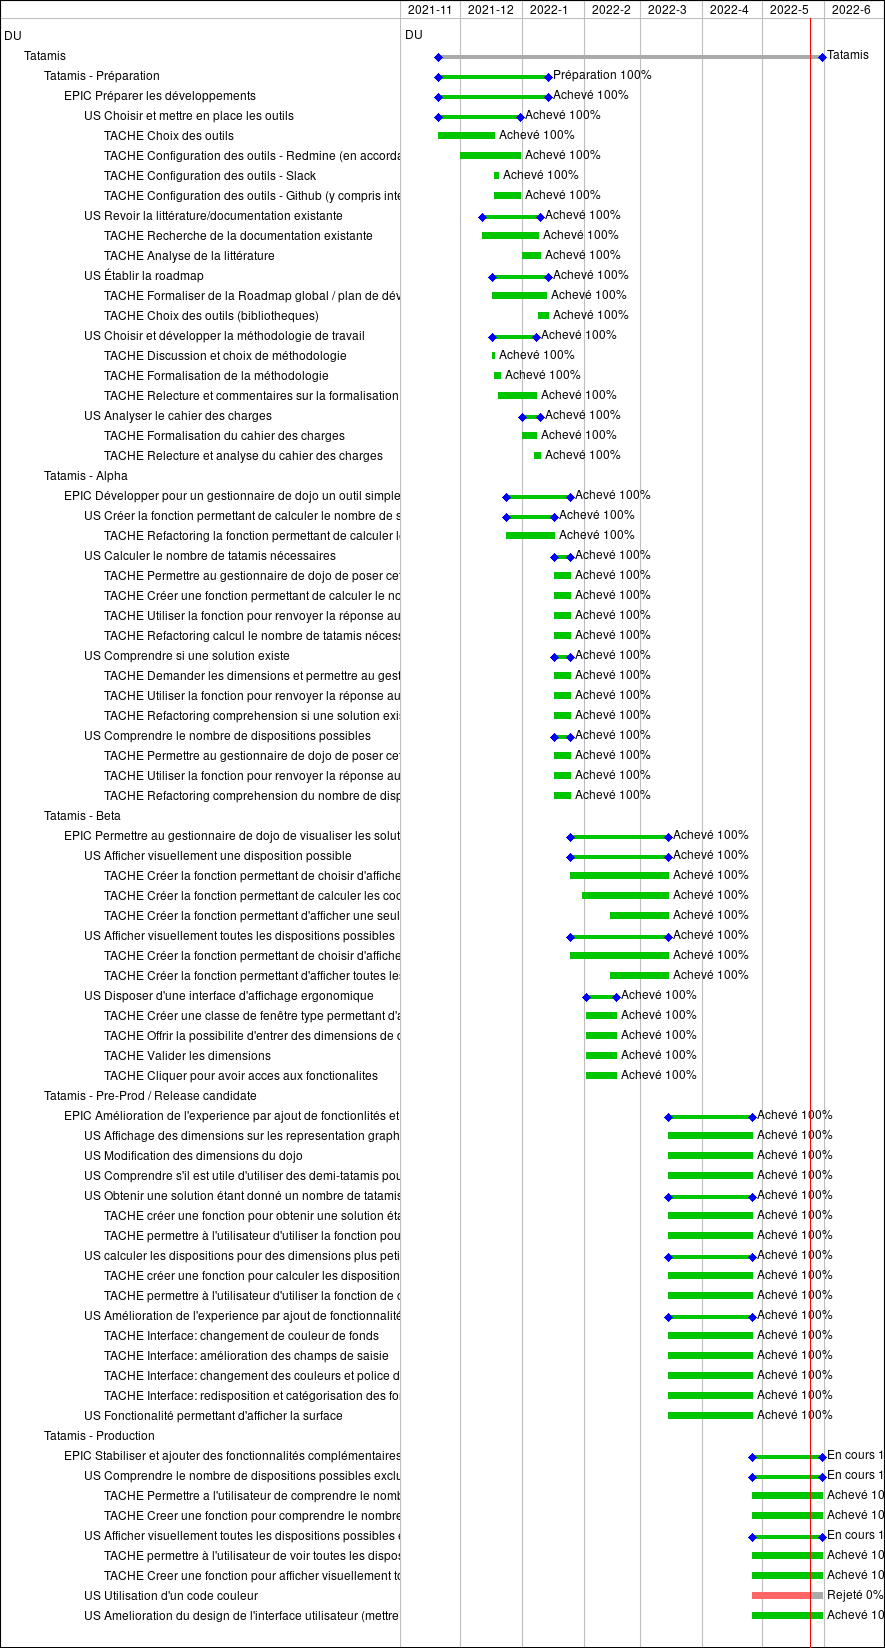
\includegraphics[height=21.5cm]{images/Gantt_final.png}
\end{center}

\chapter{Version Alpha}
\section{Backlog/roadmap du sprint Alpha}

L’objectif de ce sprint est de poser les fondations et délivrer les fonctionnalités de bases attendues par l’utilisateur, 
c'est-à- dire la compréhension des dispositions possibles et impossibles.

Pour ce faire le backlog suivant a été "embarqué" dans cette version et a résulté en la roadmap suivante:

%TODO insérer roadmap

\section{Tests}


\noindent%
\begin{adjustwidth}{-1.5cm}{0cm}

    \renewcommand{\arraystretch}{1.2}
    {\setlength{\tabcolsep}{1.5 mm}
        \begin{testtabular}{|m{0.6cm}|m{5.5cm}|m{8cm}|m{2cm}|c|} \hline
            id                                                                             & Sujet                                                                                & Test d'acceptance                                                                                        & Méthode de test & Résultat \\ \hline
            518                                                                            & TACHE Utiliser la fonction pour renvoyer la réponse au gestionnaire de dojo          &
            Quand le programme est lancé et que l'utilisateur saisi comme attendu,
            une réponse lui est renvoyée dans la console                                   & Manuel                                                                               & OK                                                                                                                                    \\ \hline
            517                                                                            & TACHE Créer une fonction permettant de calculer le nombre de tatamis nécessaires
            étant donné des dimensions de dojo et qu'une solution existe                   &
            Quand la fonction est exécutée, elle retourne le nombre de tatamis nécessaires &
            Automatisé                                                                     & OK                                                                                                                                                                                                                           \\ \hline
            \multirow{3}{0.6cm}{516}                                                       & \multirow{3}{5.5cm}{TACHE Permettre au gestionnaire de dojo de poser cette question} & 1. Quand le programme est lancé, il demande a l'utilisateur la largeur du dojo                           & Automatisé      & OK       \\ \cline{3-5}
                                                                                           &                                                                                      & 2. Quand le programme est lancé, il demande a l'utilisateur la longueur du dojo                          & Automatisé      & OK       \\ \cline{3-5}
                                                                                           &                                                                                      & 3. Quand le programme est lancé, une option est disponible pour l'utilisateur pour poser cette question. & Automatisé      & OK       \\ \hline
        \end{testtabular}}
\end{adjustwidth}


\noindent%
\begin{adjustwidth}{-1.5cm}{0cm}

    \renewcommand{\arraystretch}{1.2}
    {\setlength{\tabcolsep}{1.5 mm}
        \begin{testtabular}{|m{0.6cm}|m{5.5cm}|m{8cm}|m{2cm}|c|} \hline
            id                       & Sujet                                                                                                                                         & Test d'acceptance                                                                                                                                                                                                          & Méthode de test & Résultat \\ \hline
            515                      & TACHE Créer une fonction permettant de calculer le nombre de tatamis nécessaires étant donné des dimensions de dojo et qu'une solution existe & Quand la fonction est executée, elle retourne le nombre de tatamis nécessaires                                                                                                                                             & Automatisé      & OK       \\ \hline

            \multirow{3}{0.6cm}{514} & \multirow{3}{5.5cm}{TACHE Permettre au gestionnaire de dojo de poser cette question}                                                          & 1. Quand le programme est lancé, il demande à l'utilisateur la largeur du dojo                                                                                                                                             & Automatisé      & OK       \\ \cline{3-5}
                                     &                                                                                                                                               & 2. Quand le programme est lancé, il demande à l'utilisateur la longueur du dojo                                                                                                                                            & Automatisé      & OK       \\ \cline{3-5}
                                     &                                                                                                                                               & 3. Quand le programme est lancé, une option est disponible pour l'utilisateur pour poser cette question.                                                                                                                   & Automatisé      & OK       \\ \hline
            \multirow{2}{0.6cm}{513} & \multirow{2}{5.5cm}{US Comprendre le nombre de dispositions possibles}                                                                        & \cellcolor{tsgrey} 1. Étant donné que l'utilisateur saisie des dimensions de dojo, quand il saisie 2, il obtient le nombre conformément à l'article de Ruskey et Woodcock de 2009                                        & Automatisé      & OK       \\ \cline{3-5}
                                     &                                                                                                                                               & \cellcolor{tsgrey} 2. Étant donné que l'utilisateur saisie des dimensions de dojo en inversant la longueur et la largeur, quand il saisie 2, il obtient le nombre conformement a l'article de Ruskey et Woodcock de 2009 & Automatisé      & OK       \\ \hline

            512                      & TACHE Utiliser la fonction pour renvoyer la réponse au gestionnaire de dojo	Alpha                                                              & Quand le programme est lancé et que l'utilisateur saisie comme attendu, une réponse lui est renvoyée dans la console                                                                                                       & Automatisé      & OK       \\ \hline
            \multirow{2}{0.6cm}{511} & \multirow{2}{5.5cm}{TACHE Demander les dimensions et permettre au gestionnaire de dojo de les saisir}                                         & 1. Quand le programme est lancée, il demande a l'utilisateur la largeur du dojo                                                                                                                                            & Automatisé      & OK       \\ \cline{3-5}
                                     &                                                                                                                                               & 2. Quand le programme est lancé, il demande a l'utilisateur la longueur du dojo                                                                                                                                            & Automatisé      & OK       \\ \hline
            \multirow{2}{0.6cm}{510} & \multirow{2}{5.5cm}{US Comprendre si une solution existe}                                                                                     & \cellcolor{tsgrey} 1. Etant donné que l'utilisateur saisie des dimensions de dojo n'ayant pas de solution, quand il saisie 1, il obtient 'Il n'existe pas de disposition possible avec des tatamis 2x1 pour ce dojo'     & Automatisé      & OK       \\ \cline{3-5}
                                     &                                                                                                                                               & \cellcolor{tsgrey} 2. Étant donné que l'utilisateur saisie des dimensions de dojo ayant au moins une disposition, quand il saisie 1, il obtient 'Il existe au moins une disposition avec des tatamis 2x1 pour ce dojo'   & Automatisé      & OK       \\ \hline
        \end{testtabular}}
\end{adjustwidth}


\noindent%
\begin{adjustwidth}{-1.5cm}{0cm}

    \renewcommand{\arraystretch}{1.2}
    {\setlength{\tabcolsep}{1.5 mm}
        \begin{testtabular}{|m{0.6cm}|m{5.5cm}|m{8cm}|m{2cm}|c|} \hline
            id                                                                                                       & Sujet                                                                                                                                  & Test d'acceptance                                                                                                                                                                  & Méthode de test & Résultat \\ \hline
            \multirow{2}{0.6cm}{509}                                                                                 & \multirow{2}{5.5cm}{US Créer la fonction permettant de calculer le nombre de solutions au problème étant donné les dimensions du dojo} & 1. Quand la fonction est exécutée, elle retourne le nombre de dispositions possibles conformément a l'article de Ruskey et Woodcock de 2009                                        & Automatisé      & OK       \\ \cline{3-5}
                                                                                                                     &                                                                                                                                        & 2. Quand la fonction est exécutée en inversant la longueur et la largeur, elle retourne le nombre de dispositions possibles conformément a l'article de Ruskey et Woodcock de 2009 & Automatisé      & OK       \\ \hline

            509                                                                                                      & EPIC Développer pour un gestionnaire de dojo un outil simple lui permettant de saisir les dimensions du dojo et
            de savoir si un solution existe, le nombre de tatamis nécessaires et le nombre de dispositions possibles & \cellcolor{tsgrey} cf. tests utilisateurs des US                                                                                     &                                                                                                                                                                                    &                            \\ \hline
            \multirow{2}{0.6cm}{480}                                                                                 & \multirow{2}{5.5cm}{US Calculer le nombre de tatamis nécessaires}                                                                      & 1. Étant donne que l'utilisateur saisit des dimensions de dojo avec une solution qui existe, quand il saisie 3, il obtient le nombre de tatamis nécessaires                        & Automatisé      & OK       \\ \cline{3-5}
                                                                                                                     &                                                                                                                                        & 2. Étant donne que l'utilisateur saisit des dimensions de dojo avec aucune disposition possible, quand il saisie 3, il obtient un message indiquant l'absence de solution          & Automatisé      & OK       \\ \hline
        \end{testtabular}}
\end{adjustwidth}



\bigskip

Les tests automatisés sont définis dans le fichier \texttt{test\_alpha.py} et \texttt{test\_interface.py}. Ils peuvent être reproduits 
en l'exécutant avec ligne de commande \texttt{python3 -m pytest}.


\section{Documentation utilisateur Alpha}

\subsection{Prérequis}
%TODO faire mise en page
Configuration et installations requises:

\begin{itemize}
    \item Python 3.9 ou supérieur
    \item Librairies Python: aucune
\end{itemize}

\subsection{Comment trouver le nombre de tatamis nécessaires pour remplir un dojo?}

Lancer le programme dans un Terminal (ligne de commande: python3 interface.py)
Entrer (dans le Terminal) la longueur et la largeur du dojo en suivant les questions posées par le programme. Nb: Vous pouvez inverser la longueur et la largeur, cela n’a pas d’importance
Répondre ‘3’ à la question du programme “Que cherchez vous?”
Interpréter la réponse:
Réponse : “Le nombre de tatamis 2x1 nécessaires pour ce dojo est : [Nombre]”. Interprétation: il existe au moins une disposition possible et vous aurez besoin d’exactement [Nombre] tatamis pour remplir le dojo.
Réponse : “Il n'existe pas de disposition possible avec des tatamis 2x1 pour ce dojo”. Interprétation: il n’existe aucune disposition possible de tatamis 2 x 1 pour remplir le dojo.

\subsection{Comment savoir s’il existe une disposition possible de tatamis pour un dojo donné?}

Lancer le programme dans un Terminal (ligne de commande: python3 interface.py)
Entrer (dans le Terminal) la longueur et la largeur du dojo en suivant les questions posées par le programme. Nb: Vous pouvez inverser la longueur et la largeur, cela n’a pas d’importance
Répondre ‘1’ à la question du programme “Que cherchez vous?”
Interpréter la réponse:
Réponse : “Il existe au moins une disposition avec des tatamis 2x1 pour ce dojo”. Interprétation: il existe au moins une disposition possible.
Réponse : “Il n’existe pas de disposition possible avec des tatamis 2x1 pour ce dojo”. Interprétation: il n’existe aucune disposition possible de tatamis 2 x 1 pour remplir le dojo. Il est dans ce cas probable de devoir utiliser des demi-tatamis pour remplir pleinement le dojo.


\subsection{Comment savoir combien il existe de dispositions possibles de tatamis pour un dojo donné?}

Lancer le programme dans un Terminal (ligne de commande: python3 interface.py)
Entrer (dans le Terminal) la longueur et la largeur du dojo en suivant les questions posées par le programme. Nb: Vous pouvez inverser la longueur et la largeur, cela n’a pas d’importance
Répondre ‘2’ à la question du programme “Que cherchez vous?”
Interpréter la réponse:
a. Réponse : “Il existe [Nombre] dispositions possibles”. Interprétation: des dispositions existent pour ce dojo et il y en a [Nombre].
b. Réponse : “Il existe 0 disposition possible”. Interprétation: il n’existe pas de disposition pour ce dojo.


\section{Explication des algorithmes et choix de programmation}

\subsection{Algorithme pour les calculs de nombre de dispositions}

Nous avons tenté deux approches pour répondre à ces fonctionnalités de base:
1. Exploitation de la bibliothèque facile écrite en python pour résoudre des problèmes en programmation par contrainte. 
La publication de Xavier Olive (ref) proposant une application de cette  bibliothèque au problème qui nous concerne, 
nous avons explorer la possibilité d’adapter le programme proposé dans la publication. Si le nombre de dispositions 
proposées lors des calculs pour des dimensions de dojo données est tout à fait cohérent avec les valeurs trouvées 
dans les autres publications traitant de ce problème, il nous est rapidement apparu que les dimensions étaient limités, 
et que le temps de calcul n’était pas satisfaisant.

2. Application de l’approche proposée par Dean Hickerson (Filling rectangular rooms with Tatami mats, 2002): %TODO ajouter note bas de page
nous avons codé le programme mathématique qu’il décrit en python.

La méthode 2 a finalement été retenue car elle a l’avantage d'être très légère et rapide en exécution. 
Elle peut notamment calculer rapidement des réponses même si les dimensions sont grandes (nous n’avons d’ailleurs par 
limites les dimensions saisies a un certain nombre).


\subsection{Choix de programmation Interface}

Pour faire à l'essentiel, il a été choisi d'utiliser le terminal pour les interactions entre l'utilisateur et le programme. 
Ce n’est évidemment pas idéal, mais cela a permis de rapidement traiter la partie interface pour se concentrer sur 
les fonctionnalités et les calculs mathématiques permettant d’y répondre.

\subsection{Choix de la structure du programme}

Il nous semble important de suivre et mettre en application des principes SOLID, et en particulier du 
‘Single Responsibility Principle’ et ‘Open-Closed Principle’. 
A ce stade, vu la simplicité du programme, ce n’est pas forcément nécessaire ni applicable de manière évidente, 
mais nous souhaitons construire des fondations solides pour la suite:
Un fichier a une fonction principale
Dans cette version alpha, nous avons 2 fichiers (un fichier de front-end interface.py et un fichier de back-end alpha.py) :
interface.py : fichier contient toutes les fonctionnalités de front-end, c’est à dire l’interface utilisateur
alpha.py : fichier qui reprend les fonctions de calculs (basiques) de back-end


\section{Challenges rencontrés et apprentissage}

\subsection{Challenges rencontrés et solutions appliquées}

Les deux challenges principaux de cette version ont été les suivants:
Challenges techniques
Bien que pas très exigeante techniquement, cette version pose les fonctionnalités de base sur lesquelles 
les versions suivantes reposent. En ce qui concerne les algorithmes, le challenge principal a été la recherche 
de la documentation qui prend du temps. Mais bien que cela ait demandé du temps, nous avons eu la chance de 
trouver beaucoup de documentation de bonne qualité sur le sujet des tatamis. Il nous a ensuite été relativement 
facile d'implémenter et tester les solutions trouvées.
Challenges organisationnels
Bien que la coopération au sein de l'équipe ait débuté en phase de pré-développement, ce sprint était le premier 
qui impliquait un travail réel sur le code qui pose forcément de nouveaux challenges. Nous avons par ailleurs perdu 
définitivement un membre de l'équipe, impliquant inévitablement plus de travail de la part des membres restants. 
Pour nous permettre de bien avancer, nous avons mis en application les principes organisationnels suivants:
Sessions de travail régulières (hebdomadaires) pour discuter des points ouverts et répartir les tâches. 
Fréquence plutôt élevée pour garder un bon rythme de travail et éviter les accoups.
Retranscription écrite claire des tâches à effectuer avec les dates butoires (et dépendances de tâches lors qu’il y en a) 
avec un Compte Rendu écrit pour chaque session de travail
Communication entre les sessions de travail (par Slack), notamment pour les discussions sur l'exécution des tâches 
pré-requises à d'autres tâches dépendantes.
Travail personnel entre les session pour accomplir les tâches
Par ailleurs, pour gérer le code, github (intégré à Slack pour recevoir les notifications lors des updates) a été utilisé. 

\subsection{Apprentissage}

Les enseignements principaux de ce sprint sont les suivants:
Le choix de méthodologie agile confirmé comme étant la bonne approche pour travailler sur le projet. 
La perte d’un membre de l'équipe aurait notamment été plus difficile à gérer si tout avait été planifié de manière rigide au départ
Le bon fonctionnement de la coopération et organisation choisie (régularité des sessions de travail, documentation des sessions 
de travail avec des tâches et dates butoires claires,...)


\chapter{Version Beta}
\section{Backlog/roadmap du sprint Beta}

L’objectif de ce sprint est de donner bien plus de valeur à l'utilisateur par:
\begin{enumerate}
    \item Une visualisation des dispositions possible (ce qui apporte bien plus à l'utilisateur que la version Alpha)
    \item Une utilisation facilité par une interface utilisateur intuitive et ergonomique.
\end{enumerate}

Pour ce faire le backlog suivant a été "embarqué" dans cette version et a résulté en la roadmap suivante:


\section{Tests}


\noindent%
\begin{adjustwidth}{-1.5cm}{0cm}

    \renewcommand{\arraystretch}{1.2}
    {\setlength{\tabcolsep}{1.5 mm}

        \begin{testtabular}{|m{0.6cm}|m{5.5cm}|m{8cm}|m{2cm}|c|} \hline
            id                       & Sujet                                                                   & Test d'acceptance                                                                                             & Méthode de test & Résultat \\ \hline
            \multirow{2}{0.6cm}{539} & \multirow{2}{5.5cm}{TACHE Cliquer pour avoir accès aux fonctionnalités} & Quand l'application est lancée, les boutons s'affichent                                                       & Manuel          & OK       \\ \cline{3-5}
            &                                                                         & Quand l'utilisateur clique sur un bouton, la fonctionnalité est activée.                                      & Manuel          & OK       \\ \hline
            \multirow{3}{0.6cm}{538} & \multirow{3}{5.5cm}{TACHE Valider les dimensions}                       & Quand l'application est lancée, seules des valeurs entières peuvent être entrées                              & Manuel          & OK       \\ \cline{3-5}
            &                                                                         & Quand l'application est lancée, les valeurs entrables sont restreintes aux valeurs dans un intervalle défini. & Manuel          & OK       \\ \cline{3-5}
            &                                                                         & Quand l'utilisateur omet ou entre 0 pour au moins une dimension, un message d'erreur s'affiche.               & Manuel          & OK       \\ \hline
        \end{testtabular}}
\end{adjustwidth}


\noindent%
\begin{adjustwidth}{-1.5cm}{0cm}

    \renewcommand{\arraystretch}{1.2}
    {\setlength{\tabcolsep}{1.5 mm}

        \begin{testtabular}{|m{0.6cm}|m{5.5cm}|m{8cm}|m{2cm}|c|} \hline
            id                       & Sujet                                                                                           & Test d'acceptance                                                                                                                                                & Méthode de test & Résultat \\ \hline
            537                      & TACHE Offrir la possibilité d'entrer des dimensions de dojo                                     & Quand l'application est lancée, une fenêtre s'ouvre avec la possibilité d'entrer les dimensions.                                                                 & Manuel          & OK       \\ \hline
            536                      & TACHE Créer la fonction permettant d'afficher toutes les solutions                              & Quand la fonction reçoit en input les coordonnées des tatamis pour une disposition dimensions, alors elle retourne un graph avec toutes les solutions possibles" & Manuel          & OK       \\ \hline
            535                      & TACHE Créer la fonction permettant d'afficher une seule solution                                & Quand la fonction reçoit en input les coordonnées des tatamis pour une disposition dimensions, alors elle retourne un graph avec une solution possible"          & Manuel          & OK       \\ \hline
            534                      & TACHE Créer la fonction permettant de calculer les coordonnées des tatamis pour une disposition & Quand la fonction reçoit en input les dimensions d'un dojo, alors elle retourne les coordonnées des tatamis pour une disposition"                                & Manuel          & OK       \\ \hline
            533                      & TACHE Créer la fonction permettant de choisir d'afficher toutes les solutions                   & Étant donné les inputs des dimensions d'un dojo, quand cette fonction est choisie, elle retourne un graph avec toutes les solutions possibles"                   & Manuel          & OK       \\ \hline
            532                      & US Disposer d'une interface d'affichage ergonomique                                             & Quand le programme est lancé, il ouvre une interface ergonomique"                                                                                                & Manuel          & OK       \\ \hline
            531                      & TACHE Créer une classe de fenêtre type permettant d'avoir un affichage reproductible            & Quand l'application est lancée, une fenêtre s'ouvre avec les bonnes (adaptées à l'écran) et memes dimensions"                                                    & Manuel          & OK       \\ \hline
            530                      & TACHE Créer la fonction permettant de choisir d'afficher une seule solution                     & Étant donné les inputs des dimensions d'un dojo, quand cette fonction est choisie, elle retourne un graph avec une seule solution possible"                      & Manuel          & OK       \\ \hline
            \multirow{2}{0.6cm}{519} & \multirow{2}{5.5cm}{EPIC Permettre au gestionnaire de dojo de visualiser les solutions}         & cf. tests utilisateurs des US                                                                                                                                    &                 & OK       \\ \cline{3-5}
            &                                                                                                 & Le nombre de solution du programme donne le meme nombre de solution que le calcul de coordonnées Tatamis                                                         & Automatisé      & OK       \\ \hline
            478                      & US Afficher visuellement toutes les dispositions possibles                                      & Étant donné des dimensions d'un dojo saisies, quand il sélectionne cette option, il obtient visuellement toutes les dispositions possibles"                      & Manuel          & OK       \\ \hline
            476                      & US Afficher visuellement une disposition possible                                               & Étant donné des dimensions d'un dojo saisies, quand il sélectionne cette option, il obtient visuellement une disposition possible"                               & Manuel          & OK       \\ \hline
        \end{testtabular}
    }
\end{adjustwidth}

\bigskip

Les tests automatisés sont définis dans le fichier \texttt{testbeta.py}. Ils peuvent être reproduits en l'exécutant avec ligne de commande 
\texttt{python3 -m pytest}.

\section{Documentation utilisateur Beta}

\subsection{Prérequis}

Configuration et installations requises:
\begin{itemize}
    \item Python 3.9 ou supérieur
    \item Librairies Python: datetime, numpy, PyQt5.QtCore, PyQt5.QtGui, PyQt5.QtWidgets, sys, time.
\end{itemize}


\subsection{Comment trouver le nombre de tatamis nécessaires pour remplir un dojo?}

\begin{enumerate}
    \item Lancer l’interface (dans le Terminal avec la ligne de commande: \texttt{python3 interface.py})
    \item Entrer dans l’interface la longueur et la largeur du dojo dans les champs prévus à cet effet.

          \emph{Nb:
              \begin{itemize}
                  \item Vous pouvez inverser la longueur et la largeur, cela n’a pas d’importance
                  \item Vous pouvez entrer un nombre de tatamis compris entre 1 et 25.
              \end{itemize}
          }
    \item Cliquer sur le bouton: “Connaître le nombre de tatamis 2x1 nécessaires pour la taille du dojo”
          \emph{ Nb: Si vous oubliez d’entrer une dimension ou si vous entrez une dimension 0,
              un message d’erreur “Erreur de saisie des dimensions. Aucune dimension ne peut avoir une valeur nulle ou vide” apparaît.}
    \item Interpréter la réponse:
          \begin{enumerate}
              \item  \textbf{Réponse}: “Le nombre de tatamis 2x1 nécessaires pour ce dojo est : [Nombre]”.
                    \textbf{Interprétation}: il existe au moins une disposition possible et vous aurez besoin d’exactement [Nombre] tatamis pour remplir le dojo.
              \item  \textbf{Réponse}: “Le nombre de tatamis 2x1 nécessaires pour ce dojo est :
                    Aucune disposition possible de tatamis 2x1 pour ce dojo”. \textbf{Interprétation}:
                    il n’existe aucune disposition possible de tatamis 2 x 1 pour remplir le dojo.
          \end{enumerate}
\end{enumerate}

\subsection{Comment savoir s’il existe une disposition possible de tatamis pour un dojo donné?}

\begin{enumerate}
    \item Lancer l’interface (dans le Terminal avec la ligne de commande: \texttt{python3 interface.py})
    \item Entrer dans l’interface la longueur et la largeur du dojo dans les champs prévus à cet effet.

          \emph{Nb:
              \begin{itemize}
                  \item Vous pouvez inverser la longueur et la largeur, cela n’a pas d’importance
                  \item Vous pouvez entrer un nombre de tatamis compris entre 1 et 25.
              \end{itemize}
          }
    \item Cliquer sur le bouton: “Savoir s’il existe une disposition pour le dojo”

          \emph{Nb: Si vous oubliez d’entrer une dimension ou si vous entrez une dimension 0,
              un message d’erreur “Erreur de saisie des dimensions.
              Aucune dimension ne peut avoir une valeur nulle ou vide” apparaît.}
    \item Interpréter la réponse:
          \begin{enumerate}
              \item \textbf{Réponse}: “Il existe au moins une disposition avec des tatamis 2x1 pour ce dojo”.
                    \textbf{Interprétation}: il existe au moins une disposition possible.
              \item \textbf{Réponse}: “Il n’existe pas de disposition possible avec des tatamis 2x1 pour ce dojo”.
                    \textbf{Interprétation}: il n’existe aucune disposition possible de tatamis 2 x 1 pour remplir le dojo.
                    Il est dans ce cas probable de devoir utiliser des demi-tatamis pour remplir pleinement le dojo.
          \end{enumerate}

\end{enumerate}

\subsection{Comment savoir combien il existe des dispositions possibles de tatamis pour un dojo donné?}

\begin{enumerate}
    \item Lancer l’interface (dans le Terminal avec la ligne de commande: \texttt{python3 interface.py})
    \item Entrer dans l’interface la longueur et la largeur du dojo dans les champs prévus à cet effet.

          \emph{Nb:
              \begin{itemize}
                  \item Vous pouvez inverser la longueur et la largeur, cela n’a pas d’importance
                  \item Vous pouvez entrer un nombre de tatamis compris entre 1 et 25.
              \end{itemize}
          }
    \item Cliquer sur le bouton: “Connaître le nombre dispositions possibles”.

          \emph{Nb: Si vous oubliez d’entrer une dimension ou si vous entrez une dimension 0,
              un message d’erreur “Erreur de saisie des dimensions.
              Aucune dimension ne peut avoir une valeur nulle ou vide” apparaît.
          }
    \item Interpréter la réponse:
          \begin{enumerate}
              \item \textbf{Réponse}: “Il existe [Nombre] dispositions possibles”.
                    \textbf{Interprétation} : il existe des dispositions pour ce dojo et [Nombre] est
                    le nombre de dispositions possibles pour remplir le dojo.
              \item \textbf{Réponse}: “Il existe 0 disposition possible”.
                    \textbf{Interprétation}: la demande est non pertinente car il n’existe pas de disposition possible
                    de tatamis 2x1 pour les dimensions du dojo.
          \end{enumerate}
\end{enumerate}


\subsection{Comment afficher une disposition?}

\begin{enumerate}
    \item Lancer l’interface (dans le Terminal avec la ligne de commande: \texttt{python3 interface.py})
    \item Entrer dans l’interface la longueur et la largeur du dojo dans les champs prévus à cet effet.

          \emph{Nb:
              \begin{itemize}
                  \item Vous pouvez inverser la longueur et la largeur, cela n’a pas d’importance
                  \item Vous pouvez entrer un nombre de tatamis compris entre 1 et 25.
              \end{itemize}
          }
    \item Cliquer sur le bouton: “Afficher une disposition”

          \emph{Nb: Si vous oubliez d’entrer une dimension ou si vous entrez une dimension 0,
              un message d’erreur “Erreur de saisie des dimensions.
              Aucune dimension ne peut avoir une valeur nulle ou vide” apparaît.
          }

    \item Une disposition s’affiche

          Ou bien le message d’erreur suivant s’affiche: “Demande impossible.
          Il n'existe pas de disposition possible avec des tatamis 2x1 pour ce dojo” apparaît,
          ce qui signifie que la demande est non pertinente car il n’existe pas de disposition
          possible de tatamis 2x1 pour les dimensions du dojo.

\end{enumerate}

\subsection{Comment afficher toutes les dispositions possibles?}


\begin{enumerate}
    \item Lancer l’interface (dans le Terminal avec la ligne de commande: \texttt{python3 interface.py})
    \item Entrer dans l’interface la longueur et la largeur du dojo dans les champs prévus à cet effet.

          \emph{Nb:
              \begin{itemize}
                  \item Vous pouvez inverser la longueur et la largeur, cela n’a pas d’importance
                  \item Vous pouvez entrer un nombre de tatamis compris entre 1 et 25.
              \end{itemize}
          }
    \item Cliquer sur le bouton: “Afficher toutes les dispositions possibles”

          \emph{Nb: Si vous oubliez d’entrer une dimension ou si vous entrez une dimension 0,
              un message d’erreur “Erreur de saisie des dimensions.
              Aucune dimension ne peut avoir une valeur nulle ou vide” apparaît.
          }

    \item Toutes les dispositions possibles s’affichent

          Ou bien le message d’erreur suivant s’affiche: “Demande impossible.
          Il n'existe pas de disposition possible avec des tatamis 2x1 pour ce dojo” apparaît,
          ce qui signifie que la demande est non pertinente car il n’existe pas de disposition
          possible de tatamis 2x1 pour les dimensions du dojo.

\end{enumerate}

\section{Explication des algorithmes et choix de programmation}

\subsection{Algorithme pour l’affichage des dispositions}

\subsubsection{Première solution envisagée}

La première solution envisagée afin d’afficher la disposition des tatamis comprenait l’utilisation
de la bibliothèque python facile, dont une application au pavage de surface par tatamis a été trouvée
sur le site de Xavier Olive\footnote{https://www.xoolive.org/2016/02/29/pavage-par-tatamis.html}.  La publication semblait correspondre exactement à ce que nous souhaitions,
à savoir un calcul des dispositions possibles, et un affichage graphique adapté (via la bibliothèque matplotlib ).

La bibliothèque facile permet de modéliser et résoudre un problème en programmant ses contraintes.
Les positions et les directions des tatamis constituent les variables du problème.

Les contraintes étant constituées par les assertions suivantes:

\begin{itemize}
    \item deux tatamis ne peuvent pas se chevaucher
    \item les tatamis ne sortent pas du cadre
    \item quatre tatamis ne peuvent pas se rejoindre en un point
\end{itemize}

L’utilisation des algorithmes proposés comportait néanmoins plusieurs inconvénients :

\begin{itemize}
    \item Un temps de calcul devenant rapidement bloquant pour des dimensions de dojo encore raisonnables (16 $\times$ 16).
    \item Une bibliothèque complexe à appréhender, elle-même issue d’une adaptation en python
          de fonctionnalités développées en OCaml.
\end{itemize}

Nous aurions pu nous contenter de cette solution, mais l’impossibilité d’obtenir des pavages
pour des dimensions au-delà de 16 $\times$ 16 nous a semblé rédhibitoire.

\subsubsection{Solution retenue}

Après une recherche un peu plus poussée, il s'est avéré que ce problème de pavage dit "tatamis-parfait"
fait l'objet d'une question dans un livre édité en chinois et dont la traduction anglaise proposée pour le titre
est : "Programmer's algorithm interesting topic". Les problèmes traités dans ce livre le sont initialement en Ruby et Javascript,
néanmoins un internaute chinois propose une interprétation de l'algorithme en python sur une note de
blog\footnote{https://blog.csdn.net/chenxy\_bwave/article/details/120364982}\label{chenxy}.
Celle-ci ayant été traduite en anglais\footnote{https://www.fatalerrors.org/a/programmer-s-algorithm-interesting-topic-q32-laying-method-of-tatami.html},
nous avons pu en prendre plus facilement connaissance et ainsi en exploiter les idées.\\

L'auteur de cette note propose de modéliser la pièce en la découpant selon une grille d'intervalle 1.\\

Le problème est identifié comme celui d'un parcours de graphe (arbre binaire) en profondeur d'abord.
La racine de l'arbre étant constituée par une pièce vide de tatami. Chaque nœud du graphe correspond
à un état de pavage donné, où chaque zone de la grille contient un entier correspondant au numéro du
tatami qui la recouvre. Le nombre 0 désigne alors une zone vide de tatami.\\

La pièce est donc modélisée par une matrice de dimension H*W où H désigne sa hauteur et W sa largeur.
Afin de détecter les bords de la pièce lors du parcours, la matrice est “bordée” par le nombre -1.\\

Le cœur du problème consiste à savoir si une zone de la grille peut être recouverte par un tatami.
Étant donné que nous ne voulons pas que quatre tatamis se rejoignent en même coin, le critère est donc
qu’une zone ne peut être pavée que si les trois positions de la grille situées à gauche, en haut à gauche,
et en haut ne sont pas toutes pavées par des tatamis différents.
Cette situation est traduite par l’illustration ci-dessous :\\

\begin{center}
    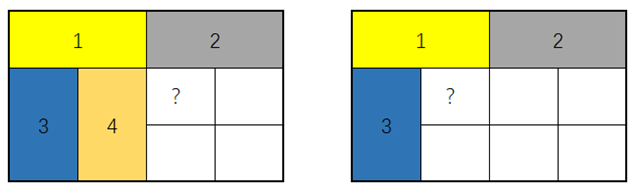
\includegraphics[width=10cm]{images/illustrationBeta-algo-2.png}
\end{center}

L’algorithme parcourt la grille ligne par ligne et colonne par colonne en vérifiant pour chaque position
si un tatamis peut-être posé : dans un premier temps en position horizontale, puis dans un deuxième temps
en position verticale. Si c’est le cas, la position de la grille ainsi que sa zone adjacente (horizontale ou verticale)
reçoivent le numéro du tatami courant et l’algorithme est appelé pour la position suivante, en incrémentant le numéro du tatami.
Lorsque la ligne atteinte correspond au bord bas du tatamis, le pavage est complet.\\

L’auteur précise qu’un tel parcours peut comporter une profondeur considérable selon les dimensions de la pièce
à paver et que selon les cas on peut donc atteindre rapidement la profondeur de récursivité maximale.\\

L'illustration d'un parcours de recherche pour un pavage (4$\times$3) est donnée ci-dessous.\\

\begin{adjustwidth}{-1.5cm}{0cm}
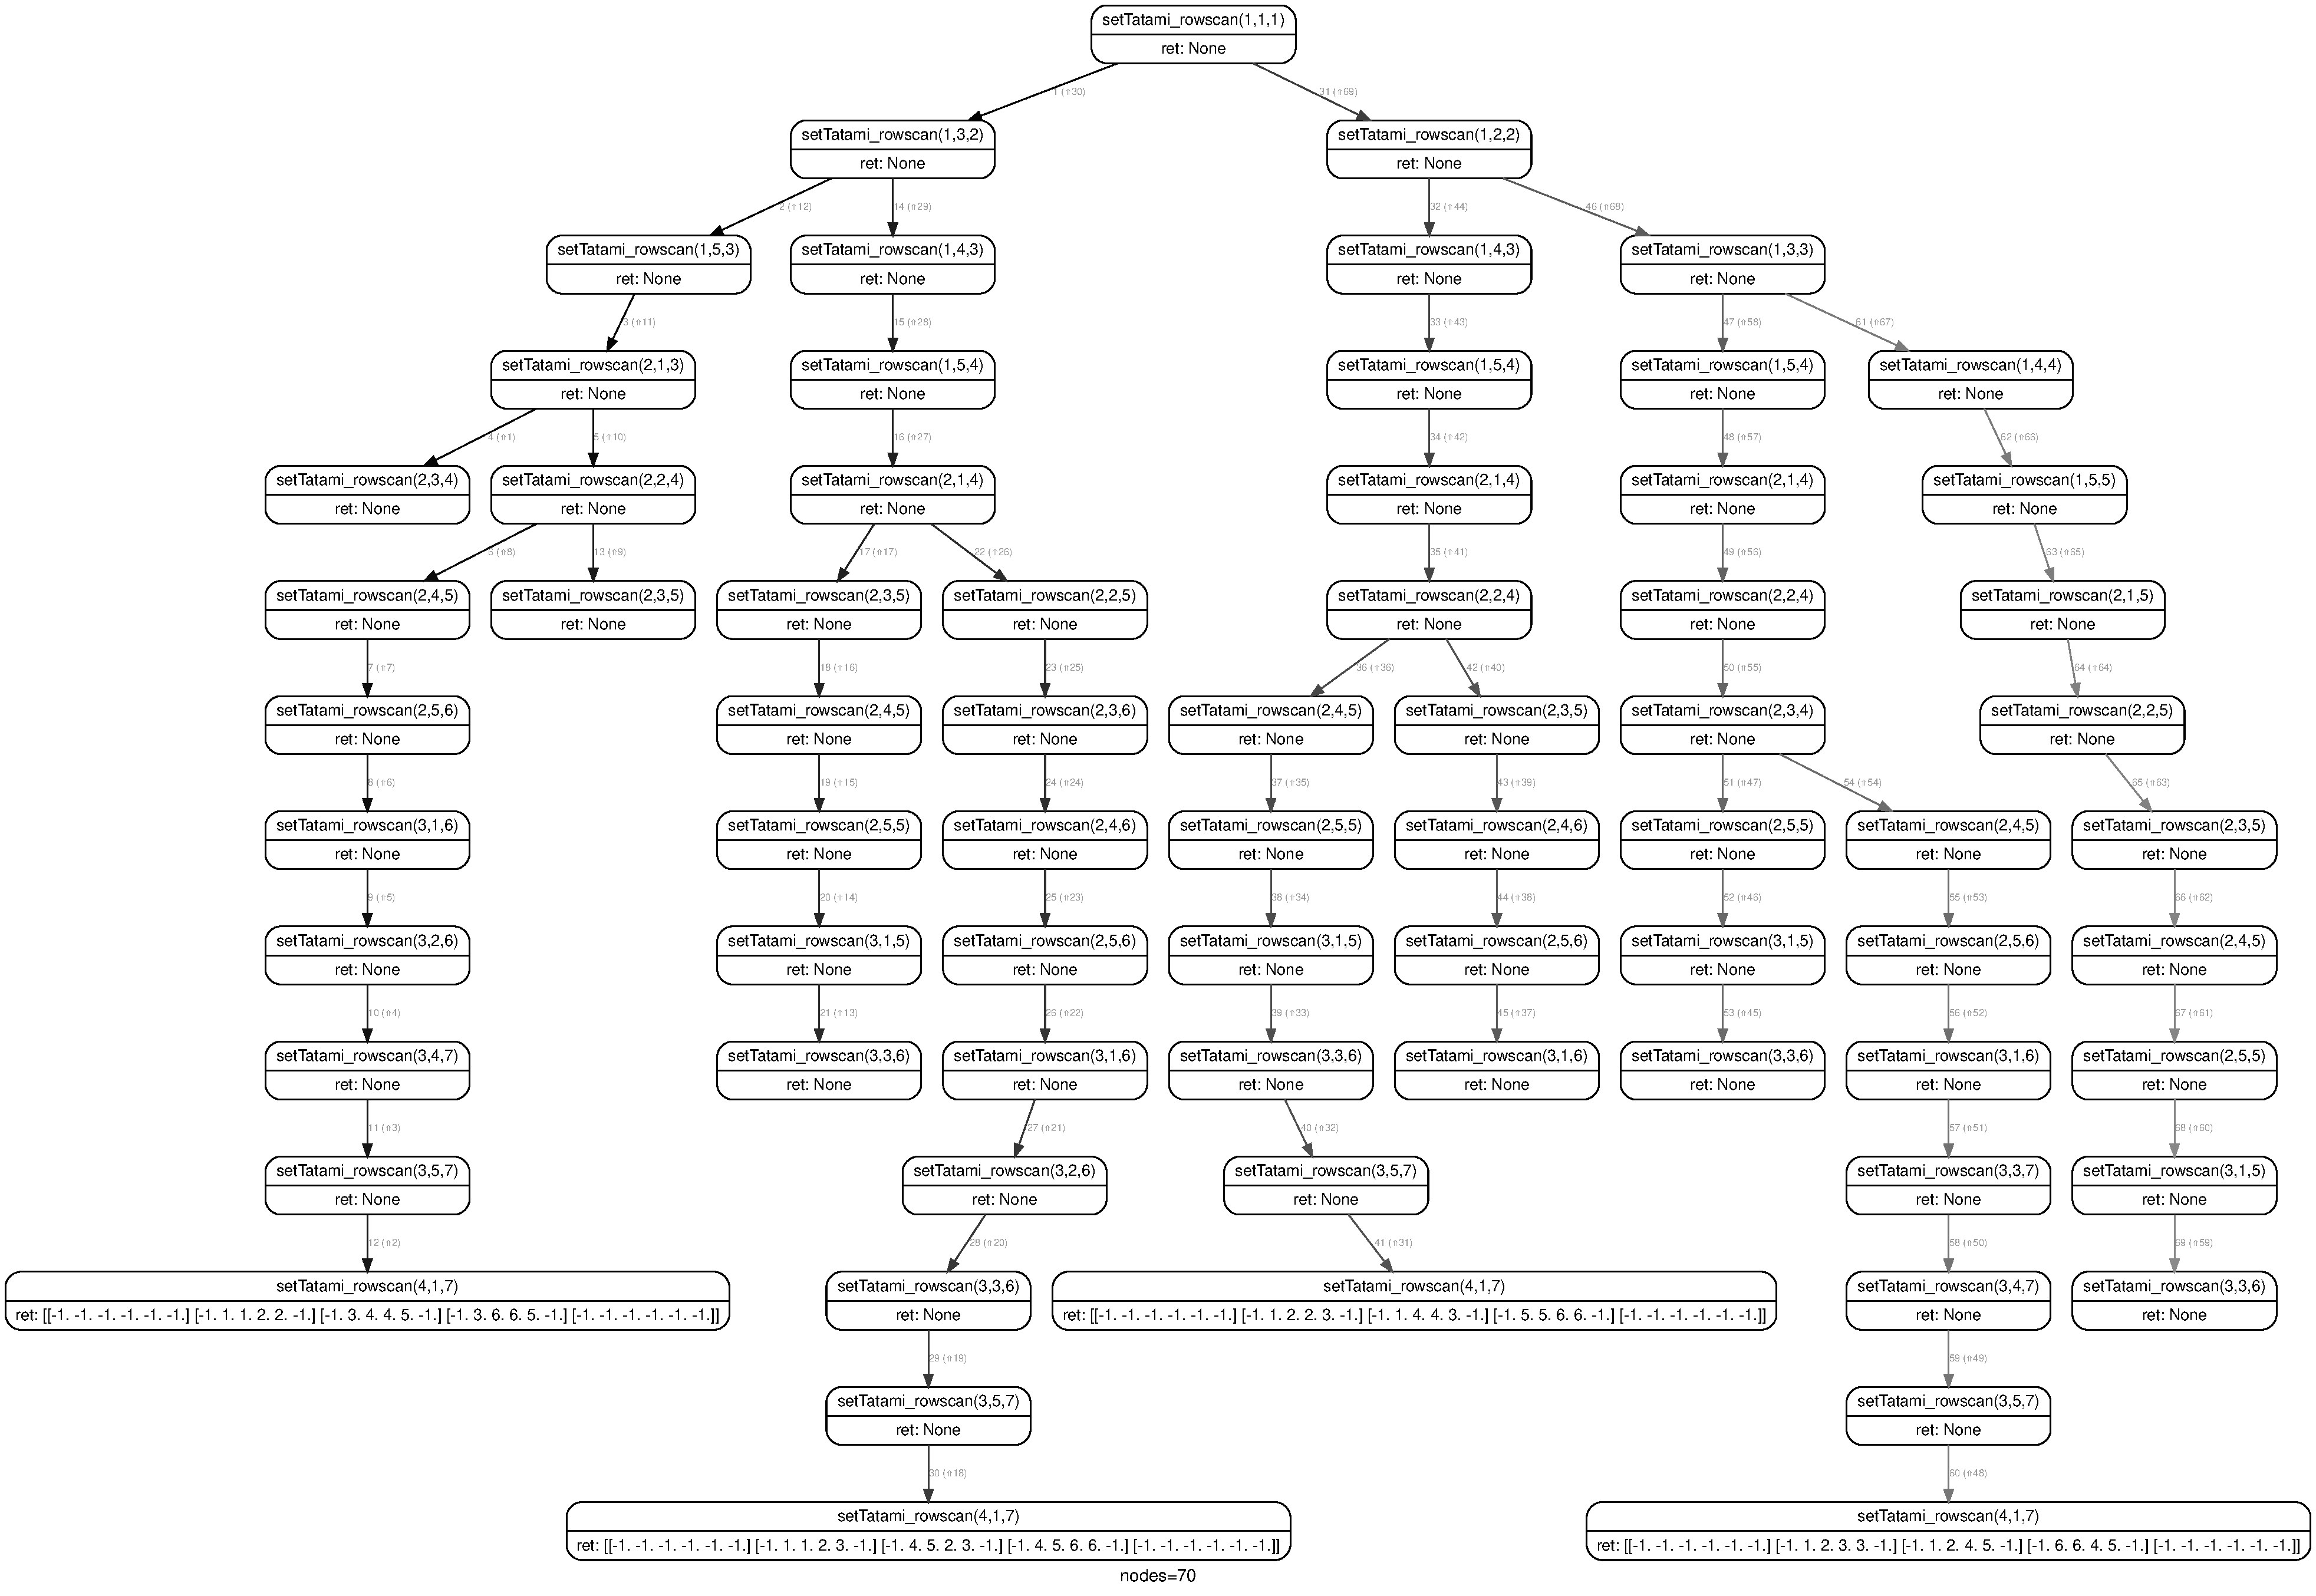
\includegraphics[width=19cm]{images/arbre4x3.pdf}
\end{adjustwidth}


En testant le programme en Python proposé par l’auteur, nous atteignons effectivement une limite de calcul,
mais celle-ci nous permet néanmoins de traiter des dojos plus grands que la solution évoquée précédemment.
Nous augmentons ainsi notre capacité de traitement d’environ 80\% puisque la dimension limite de dojo passe de 16 à 25.\\

La publication originale fournissait l’implémentation d’une fonction récursive manipulant des variables globales.
Afin de pouvoir utiliser cette solution dans notre projet, la fonction a été intégrée au sein d’une classe en tant que méthode,
et les variables globales sont devenues des attributs de celle-ci. La fonction initiale ne retournant qu’une matrice d’index,
il a fallu ajouter une méthode de classe afin de produire à partir de cette matrice, les positions de chaque tatami dans le plan.
L’enregistrement des positions se faisant à l’aide d’une liste de dictionnaire, chacun de ces dictionnaires contenant
les caractéristiques d’un tatami (index, largeur, longueur, position verticale et position horizontale).



\subsection{Choix de programmation Interface}

Les choix importants concernant l’interface ont été les suivants:


\subsubsection{Choix de la librairie d’interface graphique}

Une recherche initiale a permis d'identifier 5 librairies à notre disposition:

\begin{itemize}
    \item PyQt5
    \item Tkinter
    \item Pyside2
    \item Kivy
    \item wxPython
\end{itemize}

Trois critères de choix ont été appliqués:

\begin{itemize}
    \item Capacités de la librairie
    \item Disponibilité de la documentation et ressources en ligne
    \item Connaissances préalables par l'équipe et simplicité
\end{itemize}

L'évaluation a conclu aux résultats suivants:\\


\noindent%
\begin{adjustwidth}{-1.5cm}{0cm}

    \renewcommand{\arraystretch}{1.2}
    {\setlength{\tabcolsep}{1.5 mm}


        \begin{testtabular}{*{6}{|p{0.16\linewidth} }|} \hline

            \rowcolor{tsgrey}                               &                                                                                                & Tkinter & Pyside2 & Kivy & wxPython \\ \hline
            \cellcolor{lightgray} Capacités de la librairie & Très large variété de widgets (boutons, champs de saisie, boîtes de message…)

            Beaucoup de possibilités

            Grille disponible
            & Large variété de widgets (boutons, champs de saisie, boîtes de message…)

            Grille disponible (mais également une fonctionnalité qui facilite le placement)
            & Large variété de widgets (boutons, champs de saisie, boîtes de message…)

            Grille disponible
            & Widgets disponibles, dont certains bien designés mais d’autres moins intuitifs (par ex. les boutons)

            Grille disponible
            & Large variété de widgets (boutons, champs de saisie, boîtes de message…)

            Grille disponible
            \\ \hline

            \cellcolor{lightgray} Disponibilité de la documentation et ressources en ligne & 20 000 questions sur Stackoverflow

            & 45 000 questions sur Stackoverflow
            & 1 500 questions sur Stackoverflow
            & 12 000 questions sur Stackoverflow
            & 7 000 questions sur Stackoverflow
            \\ \hline

            \cellcolor{lightgray} Connaissances préalables et simplicité & Connaissances préalables de l'équipe & Peu de connaissances
            Mais facile a comprendre
            & Non & Non  & Non
            \\ \hline



        \end{testtabular}

    }
    % compléter tableau : disponibilité de la doc & connaissances préalables
\end{adjustwidth}

\bigskip

Compte tenu de cette évaluation, le choix entre PyQt5 et Tkinter n’a pas été évident.
Étant donné les connaissances préalables de l'équipe en PyQt5 et les possibilités plus importantes
de la librairie par rapport à Tkinter, c’est PyQt5 qui a finalement été choisi.

\subsubsection{Choix concernant la disposition des éléments de l’interface}

Deux options ont été étudiées:
Positionnement spécifique de chaque élément de l’interface (par la fonction \texttt{move()} de PyQt5)
Avantage:    Flexibilité (possibilité de placer très précisément chaque objet sur les axes abscisse et ordonnées de la fenêtre)
Inconvenient:    Fastidieux (nécessite de placer chaque objet avec ses coordonnées et les modifications de disposition - notamment par l’ajout d’objet - s’en trouve très longs à exécuter)
Positionnement par la mise en place et utilisation d’une grille (invisible à l'utilisateur) pour placer les éléments (par la sous-librairie QGridLayout de PyQt5)
Avantages:    Rapidité à coder (possibilité de placer très précisément chaque objet sur les axes abscisse et ordonnées de la fenêtre)
Bon alignement obtenu très facilement obtenu (car la grille assure le bon alignement)
Inconvenient:    Moins de flexibilité pour placer précisément les objets

Étant donné les avantages importants de l’option 2 et le fait que l’interface pour notre programme pouvait facilement être mise en place sous forme d’une grille, l’option 2 a été choisie.


\subsubsection{Choix concernant l’intuitivité de l’interface}

Pour cette première 'vraie' interface pour l’utilisateur
(sachant qu’en version Alpha, l’utilisateur interagissait avec le programme par l'intermédiaire du Terminal),
des choix importants et engageants pour la suite ont été à faire. De manière générale,
il a été choisi de mettre un focus particulier sur la facilité d’utilisation et l’intuitivité pour l’utilisateur.
Pour ce faire voilà les principales questions qui ont été étudiées et  choix effectués:

\begin{enumerate}
    \item Appel des fonctionnalités

          Pour une utilisation facile et compréhension des fonctionnalité disponible, il a été choisi
          d'utiliser des boutons pour l’appel des fonctionnalités, et de laisser beaucoup d’espace
          dans le boutons pour y afficher les fonctionnalité en détails
    \item Manière d’exprimer les retours

          Pour une qualité d’utilisation, tous les retours (message d’erreur ou réponse attendue par l’utilisateur)
          sont exprimés par des fenêtres "pop up"
    \item Guidance d’utilisation, "formation" des utilisateurs et information

          Il a été choisi de mettre un focus particulier sur ces aspects pour fournir une grande qualité de programme.
          L’objectif est de guider au maximum l’utilisateur (pour "borner" ses actions à ce qui est autorisé) et
          de fournir des messages de retour clairs pour chaque type d’erreur ou d'impossibilité d’utilisation de fonctionnalités.
          Voici les principales mesures mises en place :
          \begin{itemize}
              \item Les champs de saisie sont extrêmement guidés par une validation (à l'aide de la fonction \texttt{QIntValidator}):
                    l’utilisateur ne peut saisir que des entiers entre les valeurs inscrites sur l’interface
              \item Les seules saisies impossibles à contrôler sont la saisie de "0" ou l’absence de saisie, mais des messages d’erreur
                    ont été mis en place.
              \item Des tests sont effectués avant l’appel de chaque fonctionnalité pour savoir si la fonctionnalité est disponible avec
                    les dimensions de dojo saisies. Dans le cas contraire, un message d’erreur clair est donné à l'utilisateur.
              \item Tous les cas d’erreurs ont été traités (un utilisateur ne peut pas se retrouver bloqué en produisant une erreur
                    qui ne retourne pas une explication sur comment la résoudre)
          \end{itemize}

\end{enumerate}


\subsubsection*{Interface et messages de retour:}


\begin{itemize}
     

    \item Interface :

\begin{center}
    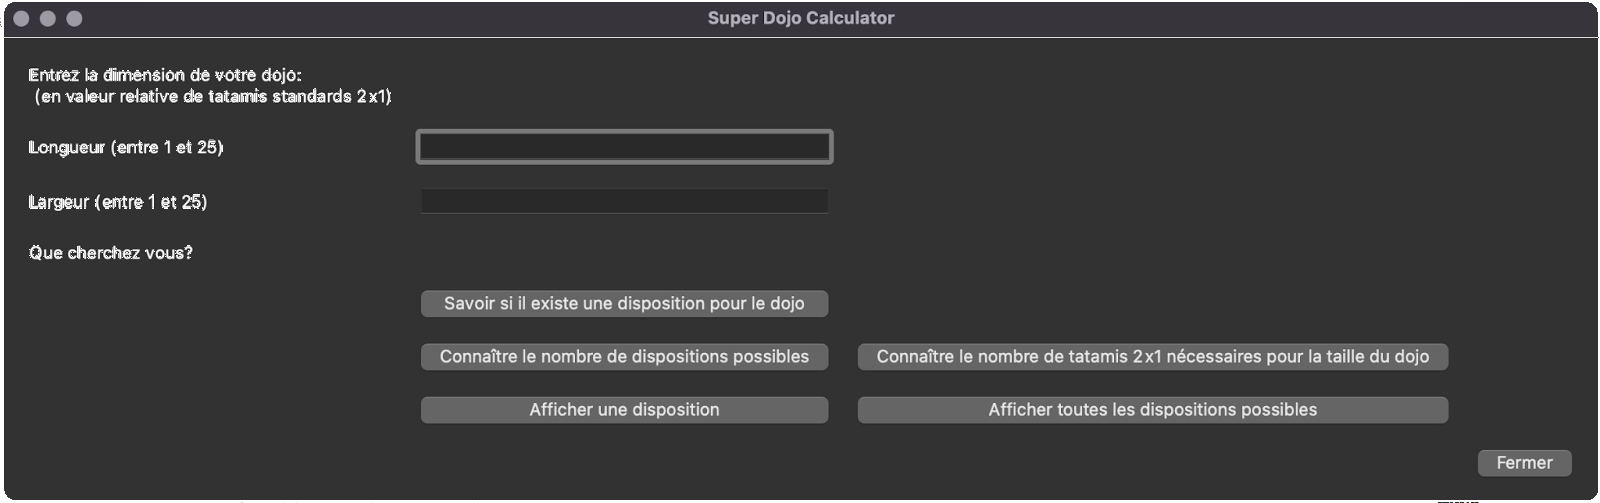
\includegraphics[scale=0.25]{images/betaInterface.png}
\end{center}


\item Exemple de message de retour (succès):

\begin{center}
    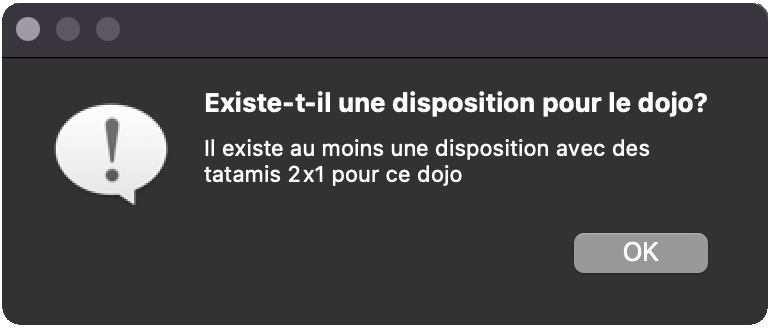
\includegraphics[scale=0.25]{images/betaRetourSucces.png}
\end{center}


\item Exemple de message indiquant à l’utilisateur que la demande est impossible avec les dimensions saisies:

\begin{center}
    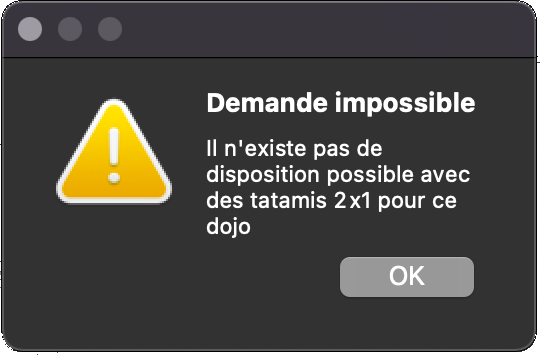
\includegraphics[scale=0.25]{images/betaImpossible.png}
\end{center}


\item Exemple de message d’erreur en cas de non saisie ou saisie nulle de dimensions:

\begin{center}
    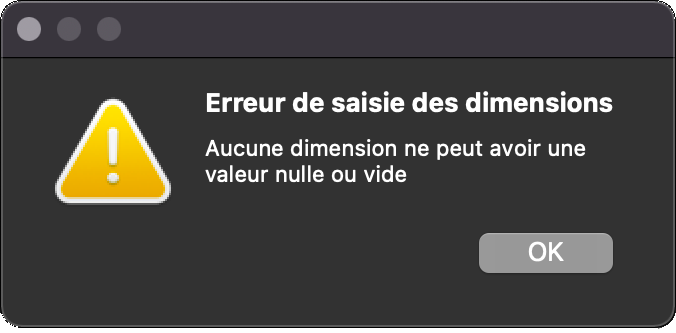
\includegraphics[scale=0.25]{images/betaErreurSaisie.png}
\end{center}


\end{itemize}

\subsection{Choix de la structure du programme}

Dans la continuité des choix fait en version Alpha, nous avons mis en application des principes \emph{SOLID}, et en particulier du
\emph{Single Responsibility Principle} et \emph{Open-Closed Principle}:

\begin{itemize}
    \item Un fichier a une fonction principale
          Dans cette version beta, nous sommes passés de 2 fichiers (un fichier de front-end \texttt{interface.py} et un fichier de back-end \texttt{alpha.py}) à
          4 fichiers du fait de la croissance des fonctionnalités et des besoins de calculs en back-end. Nous avons donc:
          \begin{itemize}
              \item \texttt{interface.py}: fichier qui continue à contenir toutes les fonctionnalités de front-end, c’est à dire l’interface utilisateur
              \item \texttt{calcul\_coordonnees\_tatamis.py}: classe qui calcule les coordonnées des tatamis d'après les dimensions du dojo.
                    Cette classe contient la fonction permettant de calculer une solution de pavage, d’après le code trouvé sur la publication
                    citée dans la partie \ref{chenxy}, à laquelle a été adjointe une fonction permettant d’obtenir les coordonnées des tatamis dans le plan.
              \item \texttt{calcul\_nombre\_dispositions.py}: fichier qui reprend les fonctions de calculs (basiques) de back-end de la version alpha.
              \item \texttt{dojo.py} : classe permettant d'instancier un tatamis d'après ces propriétés: position, dimensions, couleur. L’affichage
                    des solutions graphiques se faisant dans une fenêtre à part et utilisant des fonctions particulières, cela justifiait
                    l’existence d’une classe spécifique.
          \end{itemize}
    \item Chaque fonction a un seul usage. Plusieurs exemples peuvent être cités dans le fichier \texttt{interface.py}: de nombreuses
          fonctions à fonctionnalité très limitée mais réutilisables ont été créées comme par exemple \texttt{set\_longueur()}, \texttt{set\_largeur()}, 
          \texttt{valeur\_vide(self)}, \texttt{clickExiste()} (leur fonctionnalité est documentée dans le code et donc non-reprise dans ce rapport)

    \item Dans la mesure du possible des fonctions ou classes génériques sont créées puis réutilisées.
          Un bon exemple a cela sont les classes génériques de l’interface: \texttt{MessageSaisieInvalide}, \texttt{MessageDemandeImpossible} et \texttt{MessageInfo}.
\end{itemize}



\section{Challenges rencontrés et apprentissage}

\subsection{Challenges rencontrés et solutions appliquées}

Les deux challenges principaux de cette version ont été les suivants:
\begin{enumerate}
    \item Challenges techniques
    
          Comme on peut le constater plus dans la section sur les choix de programmation, il s’agit de la version la plus complexe techniquement.
          D’un point de vue de l’algorithme, l’affichage des dispositions a été un gros challenge technique.
          D’un point de vue de l’interface, beaucoup de choix structurants ont été nécessaires, avec des essais et révisions.
          Enfin, d’un point de vue de l’architecture du programme, les choix faits en version Alpha ont été à implémenter de manière plus poussée.
          Pour faire face à ces challenges, nous avons adopté l’approche suivante:
          \begin{itemize}
              \item Planification en systématiquement décomposant les "gros" problèmes en problèmes plus petits
              \item Recherches techniques avant tout choix à faire
              \item Revue des choix avant implémentation
          \end{itemize}
    \item Challenges organisationnels et charge de travail
    
    La charge de travail de cette version a été sous-estimée au moment de la planification et de la décision des "User story" à embarquer 
    dans cette version. En effet, la lourdeur de cette version, combinée aux choix techniques importants à faire, et à une équipe 
    de taille réduite (2 personnes) a été un challenge important.
    
    L’organisation de l'équipe et du travail est ce qui nous a permis de faire face à ce problème et de respecter le calendrier prévu. 
    Les clés de l’organisation sont restées:
    \begin{itemize}
        \item Sessions de travail pour discuter des points ouverts et repartir les taches
        \item Retranscription écrite claire des tâches à effectuer avec les dates butoir
        \item Communication entre les sessions de travail (par Slack)
        \item Travail personnel entre les session pour accomplir les tâches
    \end{itemize}

\end{enumerate}


\section{Apprentissage}

Les deux principaux apprentissages sont les suivants:

\begin{enumerate}
    \item Importance des recherches
    
    Les challenges techniques importants à surmonter nous ont permis de confirmer l’importance de faire des recherches et 
    planifier la solution avant d’implémenter. Cela évite de perdre du temps à essayer des implémentations mal pensées. 
    La réussite de cette version nous apprend également qu’avec des recherches, des problèmes qui semblent difficiles 
    peuvent être surmontés.
    \item Planifier du sprint et de la charge de travail
    
    Si cela était à refaire, nous aurions sûrement été moins ambitieux pour la version Beta en décalant des User Stories 
    à la version Release Candidate. Le travail sur cette version nous fait réaliser à la fois l'importance de bien "quantifier" 
    le volume de travail des User Stories, mais en même temps la difficulté à le faire. En effet, en particulier en ce début de projet, 
    il reste difficile d’estimer avec précision la charge de travail nécessaire à l'implémentation des User Stories.
    
    \item Promotion en classe
    
    La version alpha comporte essentiellement des algorithmes écrits sous forme de fonctions. Du fait de la complexification 
    des challenges et de l’ajout d’une interface graphique, la programmation objet s’est imposée à nous. Tout d’abord de part 
    l’utilisation de la bibliothèque PyQt et des fonctionnalités qu’il a fallu développées en s’appuyant sur celle-ci, et ensuite 
    de part les caractéristiques des solutions nécessitant d’être encapsulées et de disposer d’attribut et de fonctionnalités propres. 

\end{enumerate}


\chapter{Version Release Candidate}
\section{Backlog/roadmap du sprint Release Candidate}

L’objectif de ce sprint est de donner bien plus de valeur à l'utilisateur par l’ajout 
de nombreuses fonctionnalités supplémentaires. Un objectif secondaire a été l'amélioration 
de l’interface d’un point de vue visuel et pour en faciliter la compréhension. 

Pour ce faire le backlog suivant a été "embarqué" dans cette version et a résulté en la roadmap suivante:

\begin{center}
    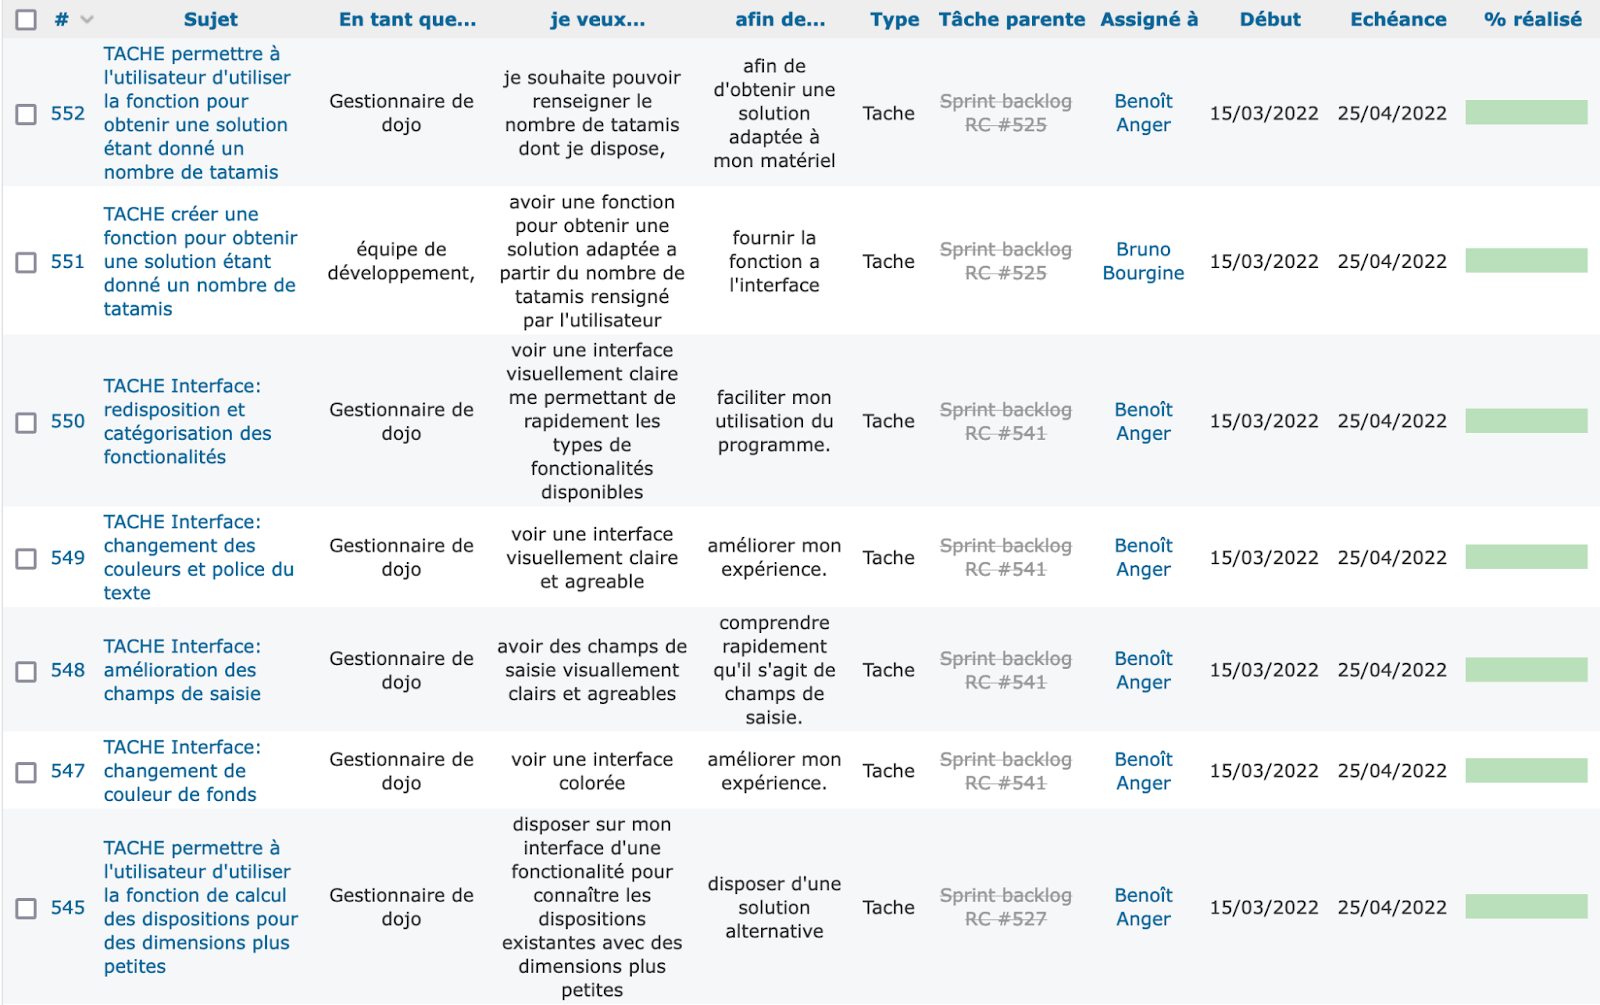
\includegraphics[width=17cm]{images/roadmap-rc-part1.png}
\end{center}

\begin{center}
    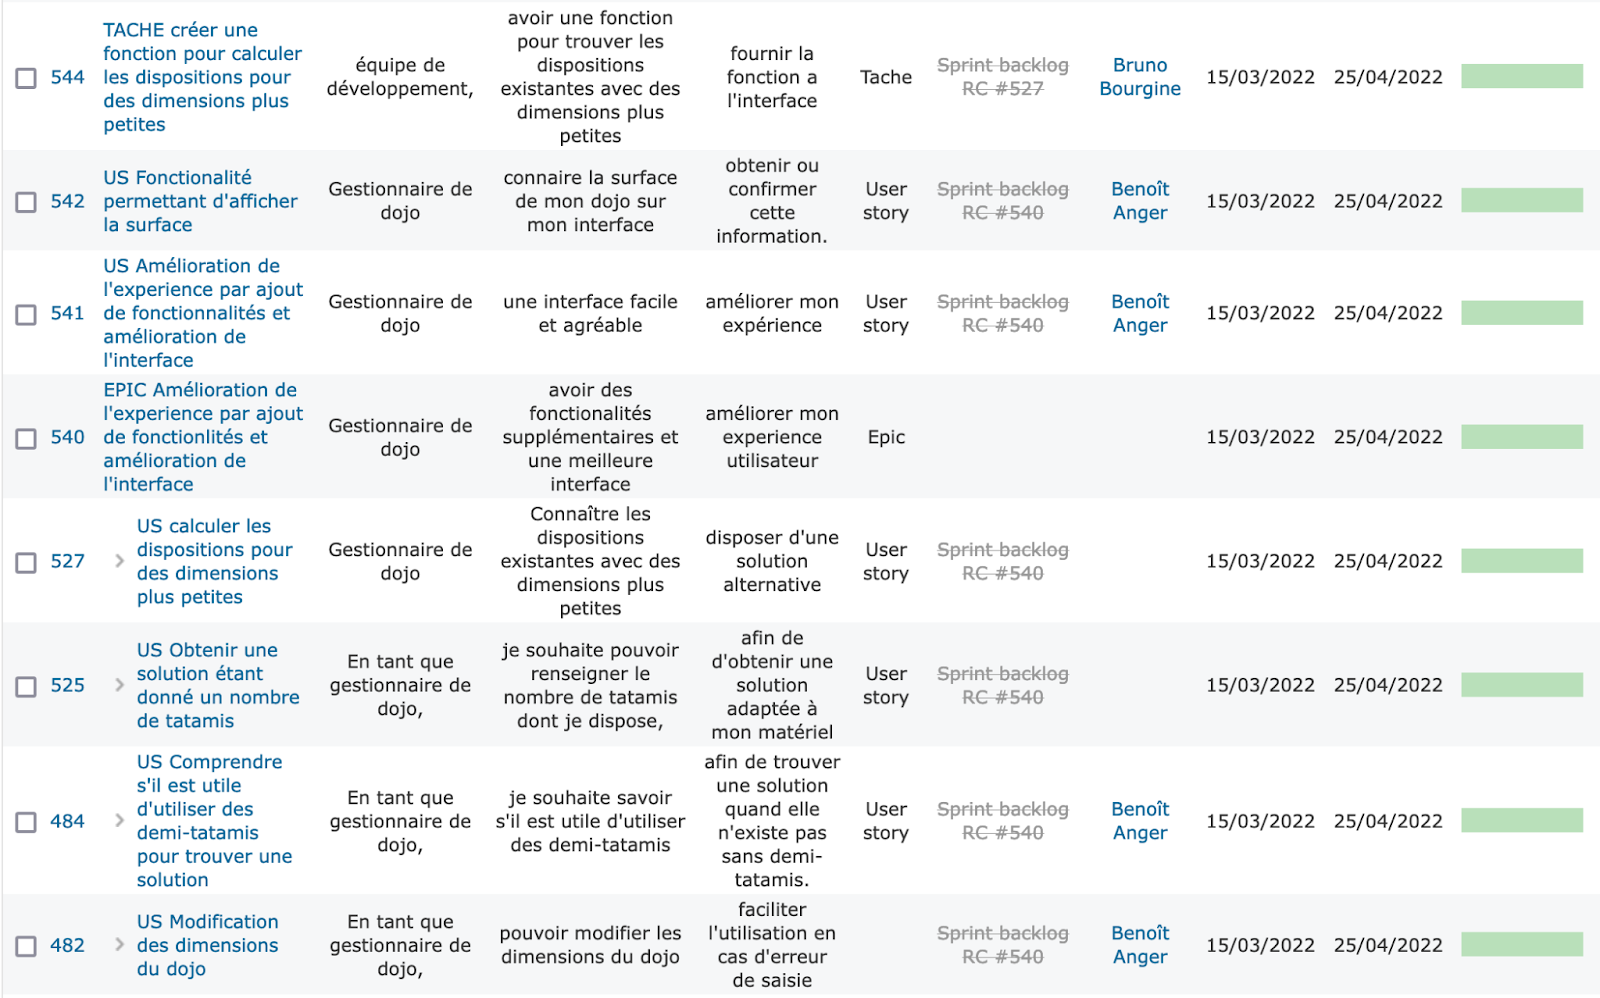
\includegraphics[width=17cm]{images/roadmap-rc-part2.png}

    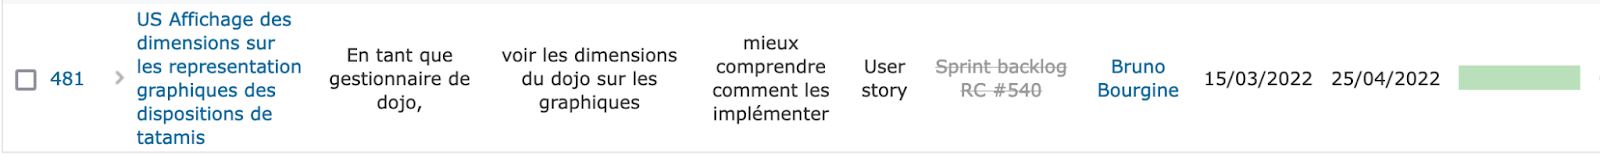
\includegraphics[width=17cm]{images/roadmap-rc-part3.png}
\end{center}


Et ici présenté en diagramme de Gantt:
\begin{center}
    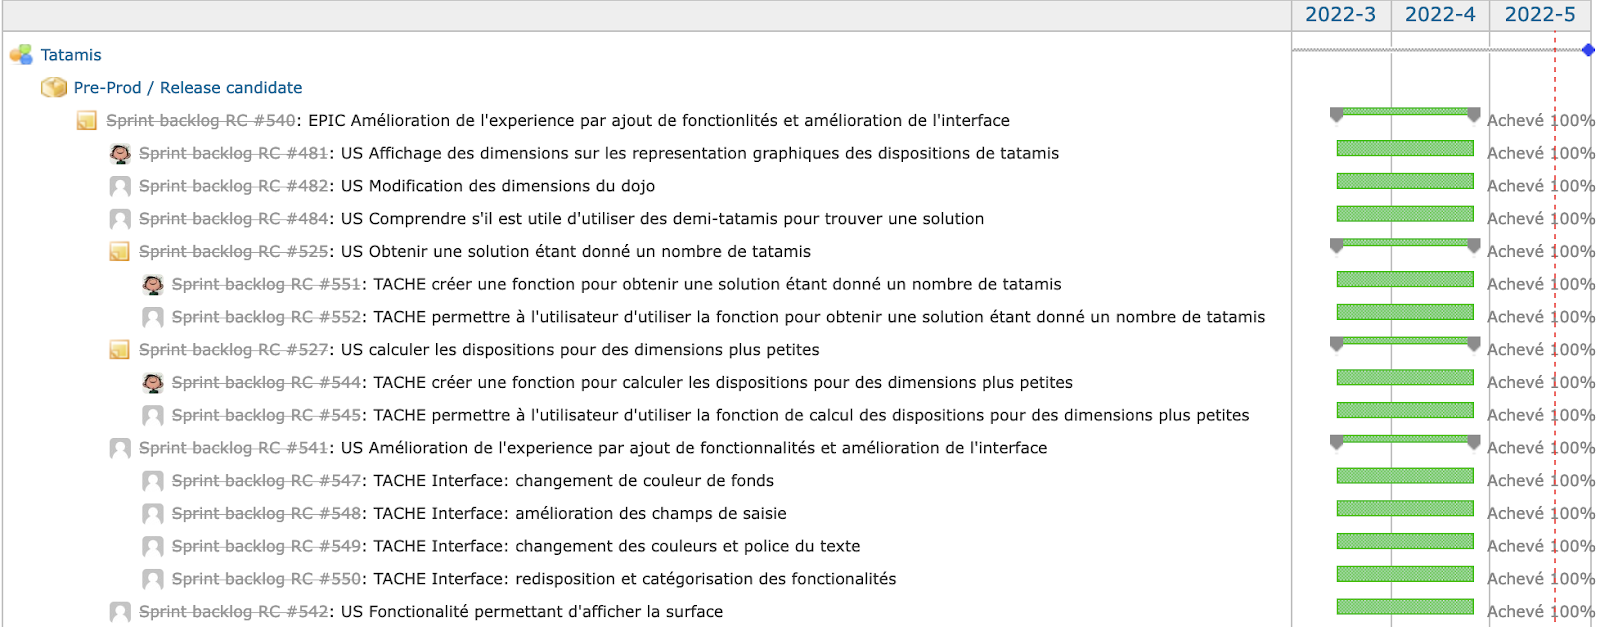
\includegraphics[width=16cm]{images/tatamis-gantt-rc.png}

\end{center}

\newpage
\section{Tests}


\noindent%
\begin{adjustwidth}{-1.5cm}{0cm}

    \renewcommand{\arraystretch}{1.2}
    {\setlength{\tabcolsep}{1.5 mm}
        \begin{testtabular}{|m{0.6cm}|m{5.5cm}|m{8cm}|m{2cm}|c|} \hline
            \rowcolor{tssteelblue} \textcolor{white}{id}                        & \textcolor{white}{Sujet}                                                                   & \textcolor{white}{Test d'acceptance (en gris : test utilisateur)}                                                                                            & \textcolor{white}{Méthode de test} & \textcolor{white}{Résultat} \\ \hline
            540 & EPIC Amélioration de l'expérience par ajout de fonctionnalités et amélioration de l'interface                      & \cellcolor{tsgrey}cf tests utilisateur des US                                                                                                                                                                                                        & Manuel          & OK       \\ \hline
            481 & US Affichage des dimensions sur les représentation graphiques des dispositions de tatamis                          & L'affichage graphique des solutions comprend un rappel des dimensions du dojo.                                                                                                                                                     & Manuel          & OK       \\ \hline
            482 & US Modification des dimensions du dojo                                                                             & L'application permet de saisir d'autres dimensions que celles initialement renseignées.                                                                                                                                            & Manuel          & OK       \\ \hline
            482 & US Modification des dimensions du dojo                                                                             & L'application permet de saisir d'autres dimensions que celles initialement renseignées.                                                                                                                                            & Manuel          & OK       \\ \hline
            484 & US Comprendre s'il est utile d'utiliser des demi-tatamis pour trouver une solution                                 & Si il n'existe pas de solutions avec des tatamis entiers, l'application affiche qu'il est toujours possible d'obtenir une solutions avec des demi-tatamis.                                                                         & Manuel          & OK       \\ \hline
            525 & US Obtenir une solution étant donné un nombre de tatamis                                                           & Lorsque l'utilisateur entre un nombre de tatamis, l'application propose une solution dont une des dimensions ne peut-être inférieure à 3 et dont le rapport largeur/longueur ne peut être inférieur à 1/3.& Manuel          & OK       \\ \hline
            551 & TACHE créer une fonction pour obtenir une solution étant donné un nombre de tatamis                                & Lorsque l'utilisateur entre un nombre de tatamis, l'application propose une solution dont une des dimensions ne peut-être inférieure à 3 et dont le rapport largeur/longueur ne peut être inférieur à 1/3.                         & Manuel          & OK       \\ \hline
            552 & TACHE permettre à l'utilisateur d'utiliser la fonction pour obtenir une solution étant donné un nombre de tatamis  & \cellcolor{tsgrey}La fonctionnalité est disponible sur l'interface utilisateur                                                                                                                                                                       & Manuel          & OK       \\ \hline
            527 & US calculer les dispositions pour des dimensions plus petites                                                      & \cellcolor{tsgrey} Lorsque l'utilisateur propose des dimensions, il n'existe pas de disposition aux dimensions plus grandes entre la(les) solution(s) alternative(s) proposée(s) par l'application et la demande de l'utilisateur. & Manuel          & OK       \\ \hline
            544 & TACHE créer une fonction pour calculer les dispositions pour des dimensions plus petites                           & Lorsque l'utilisateur propose des dimensions, il n'existe pas de disposition aux dimensions plus grandes entre la(les) solution(s) alternative(s) proposée(s) par l'application et la demande de l'utilisateur.                    & Automatisé      & OK       \\ \hline
            545 & TACHE permettre à l'utilisateur d'utiliser la fonction de calcul des dispositions pour des dimensions plus petites & \cellcolor{tsgrey}La fonctionnalité est disponible sur l'interface utilisateur                                                                                                                                                                       & Manuel          & OK       \\ \hline
            541 & US Amélioration de l'expérience par ajout de fonctionnalités et amélioration de l'interface                        & \cellcolor{tsgrey}Chaque interaction proposée par l'interface correspond à une fonctionnalité bien définie et identifiable, l'interface est intuitive est agréable visuellement.                                                                     & Manuel          & OK       \\ \hline
            547 & TACHE Interface: changement de couleur de fonds                                                                    & \cellcolor{tsgrey}Test utilisateur: Le fonds de l'interface est coloré& Manuel          & OK       \\ \hline
            548 & TACHE Interface: amélioration des champs de saisie                                                                 & \cellcolor{tsgrey}Les champs de saisie sont bien identifiables& Manuel          & OK       \\ \hline
            549 & TACHE Interface: changement des couleurs et police du texte                                                        & \cellcolor{tsgrey} Le texte est coloré et avec une police lisible et moderne& Manuel          & OK       \\ \hline
            550 & TACHE Interface: redisposition et catégorisation des fonctionnalités                                               & \cellcolor{tsgrey}Les fonctionnalités sont groupées par theme sur l'interface"& Manuel          & OK       \\ \hline
            542 & US Afficher la surface                                                                                             & \cellcolor{tsgrey} La valeur d'aire affichée sur l'interface correspond à l'aire de la surface occupée par les tatamis.& Manuel          & OK       \\ \hline
        \end{testtabular}}
\end{adjustwidth}


\section{Documentation utilisateur Release Candidate}

\subsection{Prérequis}

Configuration et installations requises:

\begin{itemize}
    \item Python 3.9 ou supérieur
    \item Librairies Python: datetime, numpy, PyQt5.QtCore, PyQt5.QtGui, PyQt5.QtWidgets, sys, time. 
    \item Installer les polices Nexa (light et bold) (fichiers otf fournis)
\end{itemize}


\subsection{Comment trouver la surface du dojo?}


\begin{enumerate}
    \item Lancer l’interface (dans le Terminal avec la ligne de commande: \texttt{python3 interface.py})
    \item Entrer dans l’interface la longueur et la largeur du dojo dans les champs prévus à cet effet.
    (Champs au bas de l’interface intitulés “Longueur (entre 1 et 25)” et “Largeur (entre 1 et 25)”). 

          \emph{Nb:
              \begin{itemize}
                  \item Vous pouvez inverser la longueur et la largeur, cela n’a pas d’importance
                  \item Vous pouvez entrer un nombre de tatamis compris entre 1 et 25.
              \end{itemize}
          }
    \item Cliquer sur le bouton: “Afficher la surface du dojo”
          \emph{ Nb: Si vous oubliez d’entrer une dimension ou si vous entrez une dimension 0,
              un message d’erreur “Erreur de saisie des dimensions. Aucune dimension ne peut avoir une valeur nulle ou vide” apparaît.}
    \item Interpréter la réponse:
          \begin{enumerate}
              \item  \textbf{Réponse}: “La surface du dojo est [Nombre]”.
                    \textbf{Interprétation}: la surface du dojo est de [Nombre] 
                    (unité identique à celle des dimensions entrées).

          \end{enumerate}
\end{enumerate}


\subsection{Comment trouver le nombre de tatamis nécessaires pour remplir un dojo?}


\begin{enumerate}
    \item Lancer l’interface (dans le Terminal avec la ligne de commande: \texttt{python3 interface.py})
    \item Entrer dans l’interface la longueur et la largeur du dojo dans les champs prévus à cet effet.
    (Champs au bas de l’interface intitulés “Longueur (entre 1 et 25)” et “Largeur (entre 1 et 25)”).

          \emph{Nb:
              \begin{itemize}
                  \item Vous pouvez inverser la longueur et la largeur, cela n’a pas d’importance
                  \item Vous pouvez entrer un nombre de tatamis compris entre 1 et 25.
              \end{itemize}
          }
    \item Cliquer sur le bouton: “Connaître le nombre de tatamis 2 $\times$ 1 nécessaires pour la taille du dojo”
          \emph{ Nb: Si vous oubliez d’entrer une dimension ou si vous entrez une dimension 0,
              un message d’erreur “Erreur de saisie des dimensions. Aucune dimension ne peut avoir une valeur nulle ou vide” apparaît.}
    \item Interpréter la réponse:
          \begin{enumerate}
              \item  \textbf{Réponse}: “Le nombre de tatamis 2x1 nécessaires pour ce dojo est : [Nombre]”.
                    \textbf{Interprétation}: il existe au moins une disposition possible et vous aurez besoin d’exactement [Nombre] tatamis pour remplir le dojo.
              \item  \textbf{Réponse}: “Demande impossible. Il n'existe pas de disposition possible avec des tatamis 2x1 pour ce dojo”. \textbf{Interprétation}:
                    il n’existe aucune disposition possible de tatamis 2 x 1 pour remplir le dojo.
          \end{enumerate}
\end{enumerate}


\subsection{Comment savoir s’il existe une disposition possible de tatamis pour un dojo donné?}


\begin{enumerate}
    \item Lancer l’interface (dans le Terminal avec la ligne de commande: \texttt{python3 interface.py})
    \item Entrer dans l’interface la longueur et la largeur du dojo dans les champs prévus à cet effet.
    (Champs au bas de l’interface intitulés “Longueur (entre 1 et 25)” et “Largeur (entre 1 et 25)”).
          \emph{Nb:
              \begin{itemize}
                  \item Vous pouvez inverser la longueur et la largeur, cela n’a pas d’importance
                  \item Vous pouvez entrer un nombre de tatamis compris entre 1 et 25.
              \end{itemize}
          }
    \item Cliquer sur le bouton: “Savoir s’il existe une disposition pour le dojo”

          \emph{Nb: Si vous oubliez d’entrer une dimension ou si vous entrez une dimension 0,
              un message d’erreur “Erreur de saisie des dimensions.
              Aucune dimension ne peut avoir une valeur nulle ou vide” apparaît.}
    \item Interpréter la réponse:
          \begin{enumerate}
              \item \textbf{Réponse}: “Il existe au moins une disposition avec des tatamis 2x1 pour ce dojo”.
                    \textbf{Interprétation}: il existe au moins une disposition possible.
              \item \textbf{Réponse}: “Il n’existe pas de disposition possible avec des tatamis 2x1 pour ce dojo”.
                    \textbf{Interprétation}: il n’existe aucune disposition possible de tatamis 2 x 1 pour remplir le dojo.
                    Il est dans ce cas probable de devoir utiliser des demi-tatamis pour remplir pleinement le dojo.
          \end{enumerate}

\end{enumerate}

\subsection{Comment savoir combien il existe de dispositions possibles de tatamis pour un dojo donné?}

\begin{enumerate}
    \item Lancer l’interface (dans le Terminal avec la ligne de commande: \texttt{python3 interface.py})
    \item Entrer dans l’interface la longueur et la largeur du dojo dans les champs prévus à cet effet.
    (Champs au bas de l’interface intitulés “Longueur (entre 1 et 25)” et “Largeur (entre 1 et 25)”). 
          \emph{Nb:
              \begin{itemize}
                  \item Vous pouvez inverser la longueur et la largeur, cela n’a pas d’importance
                  \item Vous pouvez entrer un nombre de tatamis compris entre 1 et 25.
              \end{itemize}
          }
    \item Cliquer sur le bouton: “Connaître le nombre dispositions possibles”.

          \emph{Nb: Si vous oubliez d’entrer une dimension ou si vous entrez une dimension 0,
              un message d’erreur “Erreur de saisie des dimensions.
              Aucune dimension ne peut avoir une valeur nulle ou vide” apparaît.
          }
    \item Interpréter la réponse:
          \begin{enumerate}
              \item \textbf{Réponse}: “Il existe [Nombre] dispositions possibles”.
                    \textbf{Interprétation} : il existe des dispositions pour ce dojo et [Nombre] est
                    le nombre de dispositions possibles pour remplir le dojo.
              \item \textbf{Réponse}: “Il existe 0 disposition possible”.
                    \textbf{Interprétation}: la demande est non pertinente car il n’existe pas de disposition possible
                    de tatamis 2x1 pour les dimensions du dojo.
          \end{enumerate}
\end{enumerate}


\subsection{Comment afficher une disposition?}

\begin{enumerate}
    \item Lancer l’interface (dans le Terminal avec la ligne de commande: \texttt{python3 interface.py})
    \item Entrer dans l’interface la longueur et la largeur du dojo dans les champs prévus à cet effet.
    (Champs au bas de l’interface intitulés “Longueur (entre 1 et 25)” et “Largeur (entre 1 et 25)”). 

          \emph{Nb:
              \begin{itemize}
                  \item Vous pouvez inverser la longueur et la largeur, cela n’a pas d’importance
                  \item Vous pouvez entrer un nombre de tatamis compris entre 1 et 25.
              \end{itemize}
          }
    \item Cliquer sur le bouton: “Afficher une disposition”

          \emph{Nb: Si vous oubliez d’entrer une dimension ou si vous entrez une dimension 0,
              un message d’erreur “Erreur de saisie des dimensions.
              Aucune dimension ne peut avoir une valeur nulle ou vide” apparaît.
          }

    \item Une disposition s’affiche ainsi que le rappel des dimensions du dojo, sa surface et le nombre 
    de tatamis nécessaires pour le remplir.

          Ou bien le message d’erreur suivant s’affiche: “Demande impossible.
          Il n'existe pas de disposition possible avec des tatamis 2x1 pour ce dojo” apparaît,
          ce qui signifie que la demande est non pertinente car il n’existe pas de disposition
          possible de tatamis 2x1 pour les dimensions du dojo.

\end{enumerate}

\subsection{Comment afficher toutes les dispositions possibles?}

\begin{enumerate}
    \item Lancer l’interface (dans le Terminal avec la ligne de commande: \texttt{python3 interface.py})
    \item Entrer dans l’interface la longueur et la largeur du dojo dans les champs prévus à cet effet.
    (Champs au bas de l’interface intitulés “Longueur (entre 1 et 25)” et “Largeur (entre 1 et 25)”). 

          \emph{Nb:
              \begin{itemize}
                  \item Vous pouvez inverser la longueur et la largeur, cela n’a pas d’importance
                  \item Vous pouvez entrer un nombre de tatamis compris entre 1 et 25.
              \end{itemize}
          }
    \item Cliquer sur le bouton: “Afficher toutes les dispositions possibles”

          \emph{Nb: Si vous oubliez d’entrer une dimension ou si vous entrez une dimension 0,
              un message d’erreur “Erreur de saisie des dimensions.
              Aucune dimension ne peut avoir une valeur nulle ou vide” apparaît.
          }

    \item Toutes les dispositions possibles s’affichent ainsi que le rappel des dimensions du dojo, 
    sa surface et le nombre de tatamis nécessaires pour le remplir.

          Ou bien le message d’erreur suivant s’affiche: “Demande impossible.
          Il n'existe pas de disposition possible avec des tatamis 2x1 pour ce dojo” apparaît,
          ce qui signifie que la demande est non pertinente car il n’existe pas de disposition
          possible de tatamis 2x1 pour les dimensions du dojo.

\end{enumerate}

\subsection{En cas d’absence de solutions, comment connaître la taille maximum du dojo qui permettrait de trouver au moins un disposition?}

\begin{enumerate}
    \item Lancer l’interface (dans le Terminal avec la ligne de commande: \texttt{python3 interface.py})
    \item Entrer dans l’interface la longueur et la largeur du dojo dans les champs prévus à cet effet.
    (Champs au bas de l’interface intitulés “Longueur (entre 1 et 25)” et “Largeur (entre 1 et 25)”). 

          \emph{Nb:
              \begin{itemize}
                  \item Vous pouvez inverser la longueur et la largeur, cela n’a pas d’importance
                  \item Vous pouvez entrer un nombre de tatamis compris entre 1 et 25.
              \end{itemize}
          }
    \item Cliquer sur le bouton: “Quelle taille maximum de dojo pour avoir une solution”

          \emph{Nb: Si vous oubliez d’entrer une dimension ou si vous entrez une dimension 0,
              un message d’erreur “Erreur de saisie des dimensions.
              Aucune dimension ne peut avoir une valeur nulle ou vide” apparaît.
          }

    \item Interpréter la réponse :
    \begin{enumerate}
        \item \textbf{Réponse}: “Taille maximum de dojo pour le remplir de tatamis 2 x 1. 
        La taille maximale est ([Longueur], [Largeur])”. \textbf{Interprétation}: La taille (plus petite 
        que les dimensions entrées) maximale d’un dojo pour obtenir une solution est de longueur [Longueur] et de largeur [Largeur].
        \item \textbf{Réponse}: “Demande impossible. Il existe au moins une disposition possible avec des tatamis 2x1 pour ce dojo”. 
        \textbf{Interprétation}: la demande est non pertinente car il existe au moins une disposition possible de tatamis 2x1 pour 
        les dimensions du dojo entrées. 
    \end{enumerate}
         
\end{enumerate}

\subsection{En cas d’absence de solutions, existe-t-il une solution avec des demi-tatamis?}


\begin{enumerate}
    \item Lancer l’interface (dans le Terminal avec la ligne de commande: \texttt{python3 interface.py})
    \item Entrer dans l’interface la longueur et la largeur du dojo dans les champs prévus à cet effet.
    (Champs au bas de l’interface intitulés “Longueur (entre 1 et 25)” et “Largeur (entre 1 et 25)”). 

          \emph{Nb:
              \begin{itemize}
                  \item Vous pouvez inverser la longueur et la largeur, cela n’a pas d’importance
                  \item Vous pouvez entrer un nombre de tatamis compris entre 1 et 25.
              \end{itemize}
          }
    \item Cliquer sur le bouton: “Quelle taille maximum de dojo pour avoir une solution”

          \emph{Nb: Si vous oubliez d’entrer une dimension ou si vous entrez une dimension 0,
              un message d’erreur “Erreur de saisie des dimensions.
              Aucune dimension ne peut avoir une valeur nulle ou vide” apparaît.
          }

    \item Interpréter la réponse :
    \begin{enumerate}
        \item \textbf{Réponse}: “Oui”. \textbf{Interprétation}: Le dojo (aux dimensions entrées) ne peut pas 
        être rempli par des tatamis de taille 2 x 1 mais il peut l'être en combinant au moins un demi-tatamis
        (de taille 1 x 1).

        \item \textbf{Réponse}: “Demande impossible. Il existe au moins une disposition possible avec des tatamis 2x1 pour ce dojo”. 
        \textbf{Interprétation}: la demande est non pertinente car il existe au moins une disposition possible 
        sans demi-tatamis pour les dimensions du dojo entrées. 
    \end{enumerate}
         
\end{enumerate}

\subsection{Comment obtenir les tailles des dojos admettant des solutions de remplissage à partir d’un nombre de tatamis 2 x 1?}

\begin{enumerate}
    \item Lancer l’interface (dans le Terminal avec la ligne de commande: \texttt{python3 interface.py})
    \item Entrer dans l’interface le nombre de tatamis dans le champ prévu à cet effet (Champ au bas de l’interface intitulé 
    “Nombre de tatamis 2 x 1 disponibles (entre 1 et 300)”).

          \emph{Nb: Vous pouvez entrer un nombre de tatamis compris entre 1 et 300.}

    \item Cliquer sur le bouton: “Obtenir une solution étant donne un nombre de tatamis”

          \emph{Nb: Si vous oubliez d’entrer une dimension ou si vous entrez une dimension 0,
              un message d’erreur “Erreur de saisie des dimensions.
              Aucune dimension ne peut avoir une valeur nulle ou vide” apparaît.
          }

    \item Interpréter la réponse :
    \begin{enumerate}
        \item \textbf{Réponse}: “Dimension(s) possible(s) du dojo étant donné le nombre de tatamis saisis” suivi 
        d’une liste de dimensions (couple de nombre de forme (longeur, largeur)).
        \textbf{Interprétation}: Les dimensions de dojos affichées sont des dimensions possibles de dojo permettant 
        de remplir le dojo avec le nombre de tatamis 2 x 1 saisi.

        Nb: toutes les solutions de dimensions respectent:
        \begin{itemize}
            \item Un ratio maximum de 3 entre la longueur et la largeur
            \item Une utilisation au minimum de 75\% du nombre de tatamis
        \end{itemize}

        \item \textbf{Réponse vide} (“Dimension(s) possible(s) du dojo étant donné le nombre de tatamis saisi” 
        sans dimensions affichées en dessous). \textbf{Interprétation}: il n’existe pas de dimensions de dojo 
        permettant de le remplir avec le nombre de tatamis 2 x 1 saisi (et en respectant les conditions précédemment mentionnées).

    \end{enumerate}
         
\end{enumerate}

\section{Explication de(s) algorithme(s) et choix de programmation}

\subsection{Algorithmes}

La première fonctionnalité à implémenter fut le calcul de la taille maximum du dojo qui permettrait de trouver au moins une disposition 
dans le cas ou les dimensions fournies initialement ne le permettent pas. Pour cela on fait appelle à la fonction calculant le nombre 
de disposition pour un couple de dimensions données. Tant que le nombre de disposition est nul, la largeur ou la longueur est décrémentée. 
La dimension décrémentée est choisie de façon à maximiser le nombre la surface du dojo.\\

Pour déterminer les dimensions de dojos possibles pour un nombre de tatamis donné, il a fallu dans un premier temps implémenter 
une fonction \texttt{multiples} permettant de déterminer les multiples d’un entier. Les couples de multiples ainsi obtenus constituent alors des dimensions 
de dojo proposables. Néanmoins les valeurs obtenues ne permettent pas forcément un pavage tel qu’il est souhaité, de plus, de nombreux 
couples de valeurs ne sont pas pertinents pour les dimensions d’un dojo de part leur ratio trop élevé entre longueur et largeur.\\

Afin d’obtenir des couples en plus grand nombre et avec des valeurs pertinentes, une fonction \texttt{multiples\_inf} a été implémentée permettant de sélectionner 
les multiples d’entiers inférieurs à un entier donné.  Un ratio minimum de 3 entre les valeurs du couple a été choisi, ainsi qu’un produit 
des valeurs représentant au moins 75\% de l’entier donné. Ainsi on s’assure que les dimensions obtenues soient pertinentes pour la mise en 
place du dojo.\\

Enfin, la fonction principale \texttt{recherche\_disposition} fait appel aux fonctions précédemment décrites :
\begin{itemize}
    \item La fonction \texttt{multiples\_inf} est appelée pour obtenir une liste de dimensions acceptables d’un dojo pour un nombre de tatamis donné.
    \item La fonction \texttt{recherche\_disposition\_max} est alors appelée sur chaque élément (couple) de cette liste et retourne donc un couple de 
    valeurs inférieures ou égales. Les valeurs retournées sont ajoutées à une liste.
    \item Finalement, une boucle effectue un test sur la liste de couples de valeurs obtenues afin d’en éliminer les éventuels doublons.
\end{itemize}



\subsection{Choix de programmation Interface}

Outre l’ajout à l'interface des quatre boutons correspondants aux nouvelle fonctionnalités, 
les principaux changements ont été effectués à l’interface:

\begin{itemize}
    \item Repositionnement des boutons et fonctionnalités: avec l’ajout de quatre fonctionnalités 
    pour cette version, la compréhension commence à devenir compliquée pour l’utilisateur. 
    Pour faciliter la navigation et l’utilisation, les choix suivants ont été fait:
    \begin{itemize}
        \item Création de blocs visuel pour regrouper les fonctionnalités qui se rapprochent 
        (en utilisant l’encadrement des textes pour arriver à l'effet souhaité)
        \item Séparation visuelle de la fonctionnalité ajouté nécessitant la saisie d’une nouvelle 
        donnée (en ajoutant une ligne vide dans la grille)
    \end{itemize}

    \item Travail graphique pour améliorer le rendu visuel et utilisation des possibilités offertes par PyQt5
    
    \begin{itemize}
        \item  Couleur du fond avec un dégradé de couleurs
        \item Couleur et forme des boutons
        \item Changement de la police et modification des couleurs des textes
    \end{itemize}
\end{itemize}


\begin{center}
    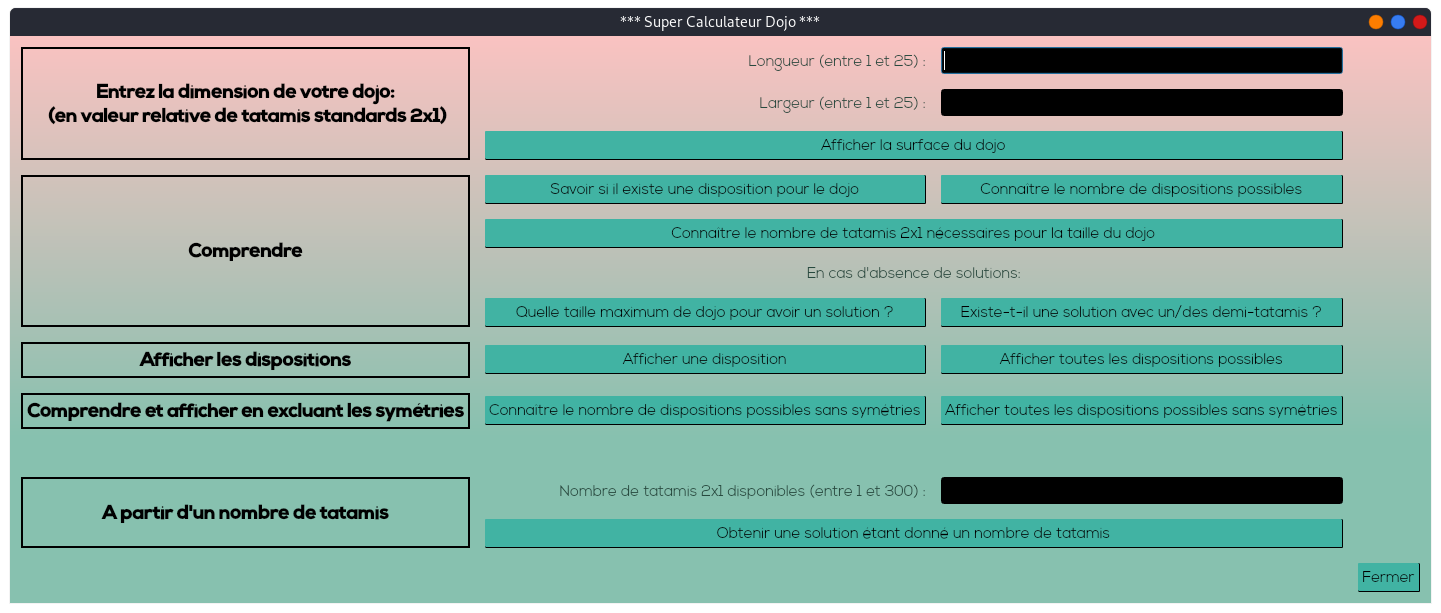
\includegraphics[width=16cm]{images/releaseInterface2.png}
\end{center}

\subsection{Choix de la structure du programme}

Dans la continuité de l’application des principes \emph{SOLID}, en particulier la volonté qu’un fichier 
ait une fonction principale, un fichier supplémentaire a été créé \texttt{release.py}. 
L’objectif de ce fichier est d'héberger les fonctionnalités implémentées spécifiquement pour 
cette version, à savoir :
\begin{itemize}
    \item le calcul de solutions pour des dimensions plus petites en cas d’impossibilité de 
    pavage avec les premières dimensions fournies par l’utilisateur.
    \item la fonction de calcul permettant de connaître les dimensions possibles de dojos 
    pour un nombre de tatamis donné.
\end{itemize}

\section{Challenges rencontrés et apprentissage}

\subsection{Challenges rencontrés et solutions appliquées}

Les deux challenges principaux de cette version ont été les suivants:
\begin{itemize}
    \item Charge de travail du sprint. Malgré avoir réalisé lors du précédent Sprint 
    l’importance de ne pas sous-estimer la charge de travail pour un sprint, nous avons eu 
    une nouvelle fois des difficultés dans cet exercice. Nous avons pourtant essayé de bien 
    planifiée (cf. partie suivante ‘Apprentissage’) mais avec 4 fonctionnalités et des travaux 
    sur l’interface, nous avons encore une fois été très ambitieux. La raison est en particulier 
    due au fait que 2 des fonctionnalités ont nécessité des efforts importants sur l'algorithme.
    \item Challenges techniques pour les fonctionnalités:
    \begin{itemize}
        \item Taille maximum d’un dojo ayant des disposition(s) possible(s) (en cas d’absence 
        de solution pour le dojo aux dimensions saisies par l’utilisateur)
        \item Obtention de dimensions de dojos (avec solutions) étant donné un nombre de tatamis 
        saisis par l’utilisateur. Cette fonctionnalité a été particulièrement difficile car les 
        possibilités sont multiples et des critères de sélection ont dû être ajoutés. Une recherche 
        de doublons a également dû être appliquée.
    \end{itemize}
\end{itemize}

\subsection{Apprentissage}

Le principal apprentissage est la phase de préparation et priorisation des User Stories 
à \emph{embarquer} dans la version.

Étant donné les challenges rencontrés lors du précédent Sprint, nous avons décidé de mieux planifier 
les 2 derniers Sprint et avons procédé ainsi:
\begin{itemize}
    \item Liste des fonctionnalités/User stories potentielles
    \item Travaux de recherche et estimation de la complexité selon 2 dimensions: effort sur 
    l'algorithme et effort sur l’interface. Efforts dimensionnés en 3 catégories: faible, moyen et élevé
    \item Décisions sur les User stories pour les 2 derniers Sprint en essayant d'équilibrer la charge de travail.
\end{itemize}
Bien que nous ayons à nouveau sur-dimensionné le Sprint Release Candidate, nous sommes satisfait 
de la méthodologie de planification appliquée. Notre erreur se trouve au niveau de l’estimation 
de l’effort, probablement dû à notre manque d'expérience de la programmation. Pour le dernier Sprint, 
nous essayerons de compenser notre manque d'expérience par une réflexion plus approfondie du travail 
à effectuer pour achever la User Story.



\chapter{Version Production}
\section{Backlog/roadmap du sprint Production}

L’objectif de ce sprint est de finaliser en augmentant encore la valeur donné à l'utilisateur par: 
Ajout de deux fonctionnalités concernant les dispositions symétriques. L’objectif étant d'éliminer ces dispositions symétriques qui apportent peu, voire prêtent à confusion pour l’utilisateur.
Dernière amélioration mineure de l’interface, surtout sur le visuel, pour aligner le design des messages de réponse à celui de l’interface principale.

Pour ce faire le backlog suivant a été \emph{embarqué} dans cette version et a résulté en la roadmap suivante:

\section{Tests}

Les tests réalisés pour cette version et leurs résultats sont les suivants:

%TODO inclure tableaux tests

Par ailleurs, étant donné qu’il s’agit de la dernière version pour mise en production, 
il est important de tester l’ensemble des fonctionnalités du programme. Des tests de non régression 
ont été effectués:

%TODO inclure tableaux tests non regression

Erreur sur validation des saisies:
Une erreur a été constaté suivant les versions utilisés de PyQt:
\begin{itemize}
    \item Version 5.9.7: la validation de la saisie des données fonctionne (comportement attendu)
    \item Version 5.12.2: la validation fonctionne partiellement (cela limite bien le type d'entrée - uniquement des entiers, et limite le nombre de chiffres, mais cela ne limite pas à 25 ou 300 comme attendu; cela limite uniquement à respectivement 99 et 999). Pour corriger ce changement de comportement de QIntValidator, un nouveau message d’erreur a été mis en place.
\end{itemize}

\section{Documentation Utilisateur Production}

\subsection{Prérequis}

Configuration et installations requises:

\begin{itemize}
    \item Python 3.9 ou supérieur
    \item Librairies Python: datetime, numpy, PyQt5.QtCore, PyQt5.QtGui, PyQt5.QtWidgets, sys, time.
     (Idéalement la version 5.9.7 de PyQt) 
    \item Installer les polices Nexa (light et bold) (fichiers otf fournis)
\end{itemize}


\newpage


% \appendix
% \section{Annexe : version Beta}\label{appendix:beta}

% Arbre des appels récursifs pour la recherche de solutions de pavage d'un dojo de dimension 4 $\times$ 3 

% \begin{adjustwidth}{-1.5cm}{0cm}
% 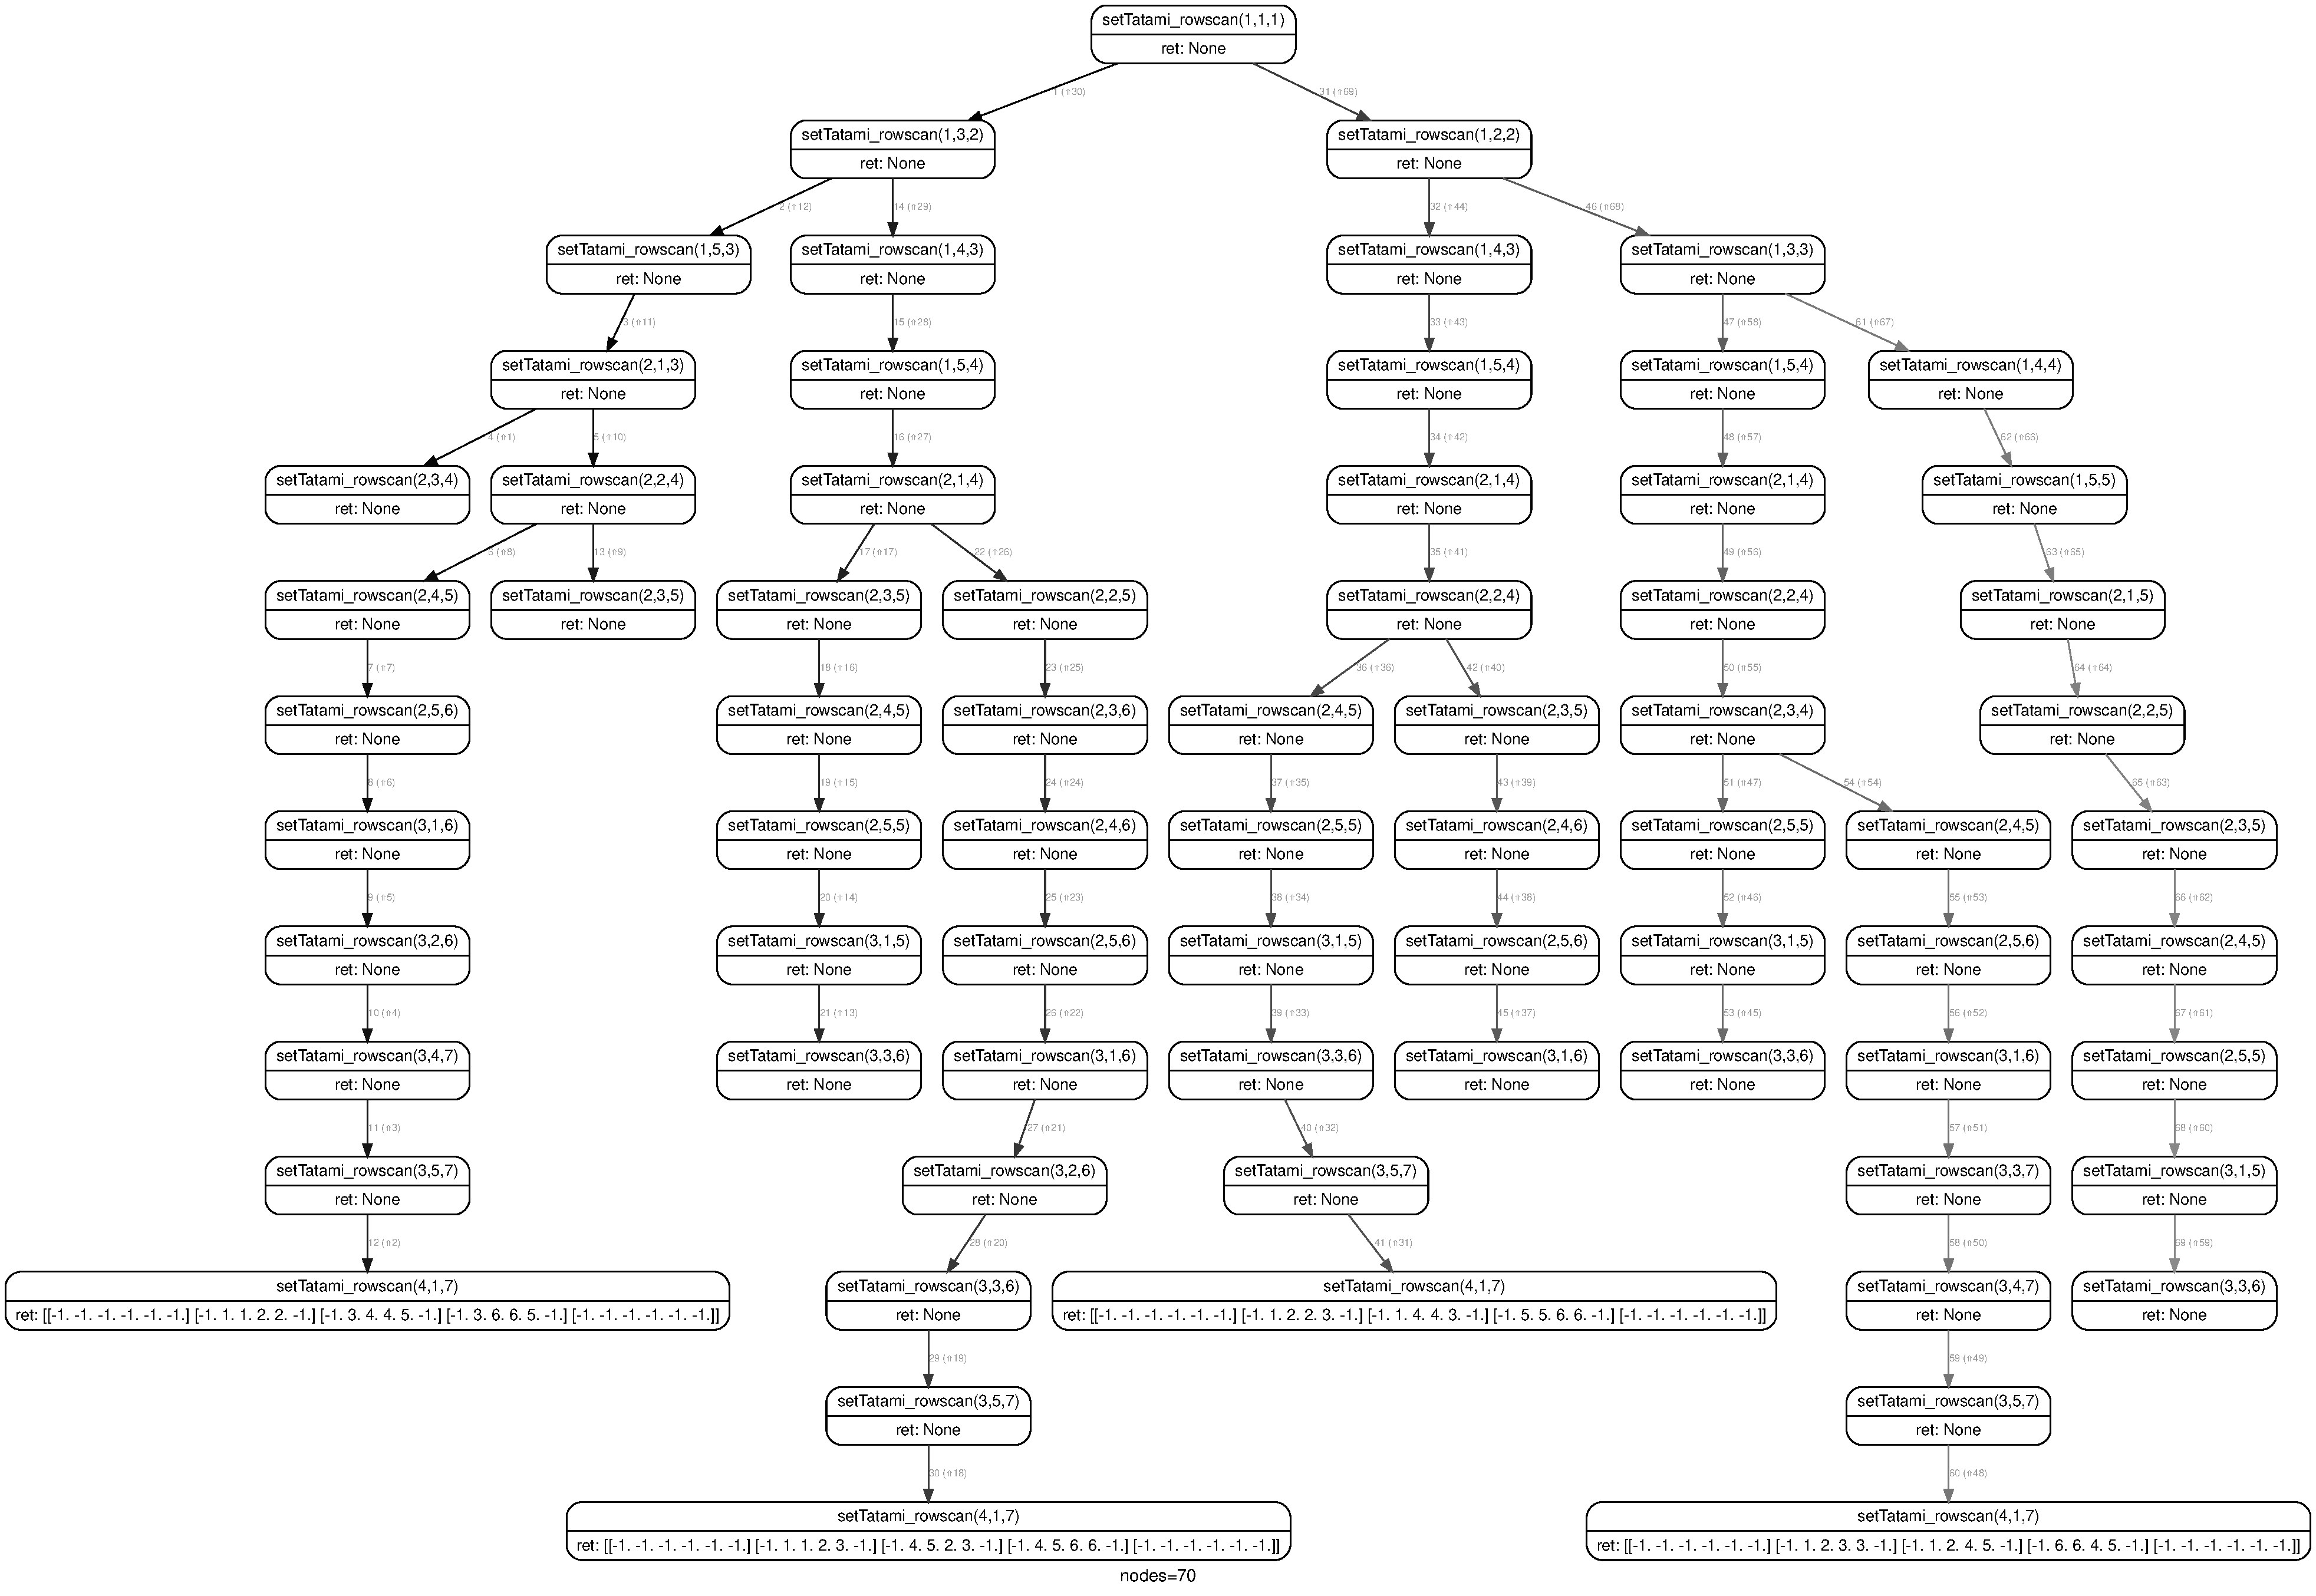
\includegraphics[width=19cm]{images/arbre4x3.pdf}
% \end{adjustwidth}
% \chapter{Tests}
% \section{Méthode et outil de test}

Les test automatisées sont réalisés à l'aide de la bibliothèque \textbf{pytest} . Les fonctions et les classes testées sont
appelées par des fonctions de test dédiées qui vérifie la concordance des valeurs retournées avec ce qui est attendu.



\section{Version Alpha}


\noindent%
\begin{adjustwidth}{-1.5cm}{0cm}

    \renewcommand{\arraystretch}{1.2}
    {\setlength{\tabcolsep}{1.5 mm}
        \begin{tabular}{|m{0.6cm}|m{5.5cm}|m{8cm}|m{2cm}|c|} \hline
            id                                                                             & Sujet                                                                                & Test d'acceptance                                                                                        & Méthode de test & Résultat \\ \hline
            518                                                                            & TACHE Utiliser la fonction pour renvoyer la réponse au gestionnaire de dojo          &
            Quand le programme est lancé et que l'utilisateur saisi comme attendu,
            une réponse lui est renvoyée dans la console                                   & Manuel                                                                               & OK                                                                                                                                    \\ \hline
            517                                                                            & TACHE Créer une fonction permettant de calculer le nombre de tatamis nécessaires
            étant donné des dimensions de dojo et qu'une solution existe                   &
            Quand la fonction est exécutée, elle retourne le nombre de tatamis nécessaires &
            Automatisé                                                                     & OK                                                                                                                                                                                                                           \\ \hline
            \multirow{3}{0.6cm}{516}                                                       & \multirow{3}{5.5cm}{TACHE Permettre au gestionnaire de dojo de poser cette question} & 1. Quand le programme est lancé, il demande a l'utilisateur la largeur du dojo                           & Automatisé      & OK       \\ \cline{3-5}
                                                                                           &                                                                                      & 2. Quand le programme est lancé, il demande a l'utilisateur la longueur du dojo                          & Automatisé      & OK       \\ \cline{3-5}
                                                                                           &                                                                                      & 3. Quand le programme est lancé, une option est disponible pour l'utilisateur pour poser cette question. & Automatisé      & OK       \\ \hline
        \end{tabular}}
\end{adjustwidth}


\noindent%
\begin{adjustwidth}{-1.5cm}{0cm}

    \renewcommand{\arraystretch}{1.2}
    {\setlength{\tabcolsep}{1.5 mm}
        \begin{tabular}{|m{0.6cm}|m{5.5cm}|m{8cm}|m{2cm}|c|} \hline
            id                       & Sujet                                                                                                                                         & Test d'acceptance                                                                                                                                                                                                          & Méthode de test & Résultat \\ \hline
            515                      & TACHE Créer une fonction permettant de calculer le nombre de tatamis nécessaires étant donné des dimensions de dojo et qu'une solution existe & Quand la fonction est executée, elle retourne le nombre de tatamis nécessaires                                                                                                                                             & Automatisé      & OK       \\ \hline

            \multirow{3}{0.6cm}{514} & \multirow{3}{5.5cm}{TACHE Permettre au gestionnaire de dojo de poser cette question}                                                          & 1. Quand le programme est lancé, il demande à l'utilisateur la largeur du dojo                                                                                                                                             & Automatisé      & OK       \\ \cline{3-5}
                                     &                                                                                                                                               & 2. Quand le programme est lancé, il demande à l'utilisateur la longueur du dojo                                                                                                                                            & Automatisé      & OK       \\ \cline{3-5}
                                     &                                                                                                                                               & 3. Quand le programme est lancé, une option est disponible pour l'utilisateur pour poser cette question.                                                                                                                   & Automatisé      & OK       \\ \hline
            \multirow{2}{0.6cm}{513} & \multirow{2}{5.5cm}{US Comprendre le nombre de dispositions possibles}                                                                        & \cellcolor{tsgrey} 1. Étant donné que l'utilisateur saisie des dimensions de dojo, quand il saisie 2, il obtient le nombre conformément à l'article de Ruskey et Woodcock de 2009                                        & Automatisé      & OK       \\ \cline{3-5}
                                     &                                                                                                                                               & \cellcolor{tsgrey} 2. Étant donné que l'utilisateur saisie des dimensions de dojo en inversant la longueur et la largeur, quand il saisie 2, il obtient le nombre conformement a l'article de Ruskey et Woodcock de 2009 & Automatisé      & OK       \\ \hline

            512                      & TACHE Utiliser la fonction pour renvoyer la réponse au gestionnaire de dojo	Alpha                                                              & Quand le programme est lancé et que l'utilisateur saisie comme attendu, une réponse lui est renvoyée dans la console                                                                                                       & Automatisé      & OK       \\ \hline
            \multirow{2}{0.6cm}{511} & \multirow{2}{5.5cm}{TACHE Demander les dimensions et permettre au gestionnaire de dojo de les saisir}                                         & 1. Quand le programme est lancée, il demande a l'utilisateur la largeur du dojo                                                                                                                                            & Automatisé      & OK       \\ \cline{3-5}
                                     &                                                                                                                                               & 2. Quand le programme est lancé, il demande a l'utilisateur la longueur du dojo                                                                                                                                            & Automatisé      & OK       \\ \hline
            \multirow{2}{0.6cm}{510} & \multirow{2}{5.5cm}{US Comprendre si une solution existe}                                                                                     & \cellcolor{tsgrey} 1. Etant donné que l'utilisateur saisie des dimensions de dojo n'ayant pas de solution, quand il saisie 1, il obtient 'Il n'existe pas de disposition possible avec des tatamis 2x1 pour ce dojo'     & Automatisé      & OK       \\ \cline{3-5}
                                     &                                                                                                                                               & \cellcolor{tsgrey} 2. Étant donné que l'utilisateur saisie des dimensions de dojo ayant au moins une disposition, quand il saisie 1, il obtient 'Il existe au moins une disposition avec des tatamis 2x1 pour ce dojo'   & Automatisé      & OK       \\ \hline
        \end{tabular}}
\end{adjustwidth}


\noindent%
\begin{adjustwidth}{-1.5cm}{0cm}

    \renewcommand{\arraystretch}{1.2}
    {\setlength{\tabcolsep}{1.5 mm}
        \begin{tabular}{|m{0.6cm}|m{5.5cm}|m{8cm}|m{2cm}|c|} \hline
            id                                                                                                       & Sujet                                                                                                                                  & Test d'acceptance                                                                                                                                                                  & Méthode de test & Résultat \\ \hline
            \multirow{2}{0.6cm}{509}                                                                                 & \multirow{2}{5.5cm}{US Créer la fonction permettant de calculer le nombre de solutions au problème étant donné les dimensions du dojo} & 1. Quand la fonction est exécutée, elle retourne le nombre de dispositions possibles conformément a l'article de Ruskey et Woodcock de 2009                                        & Automatisé      & OK       \\ \cline{3-5}
                                                                                                                     &                                                                                                                                        & 2. Quand la fonction est exécutée en inversant la longueur et la largeur, elle retourne le nombre de dispositions possibles conformément a l'article de Ruskey et Woodcock de 2009 & Automatisé      & OK       \\ \hline

            509                                                                                                      & EPIC Développer pour un gestionnaire de dojo un outil simple lui permettant de saisir les dimensions du dojo et
            de savoir si un solution existe, le nombre de tatamis nécessaires et le nombre de dispositions possibles & \cellcolor{tsgrey} cf. tests utilisateurs des US                                                                                     &                                                                                                                                                                                    &                            \\ \hline
            \multirow{2}{0.6cm}{480}                                                                                 & \multirow{2}{5.5cm}{US Calculer le nombre de tatamis nécessaires}                                                                      & 1. Étant donne que l'utilisateur saisit des dimensions de dojo avec une solution qui existe, quand il saisie 3, il obtient le nombre de tatamis nécessaires                        & Automatisé      & OK       \\ \cline{3-5}
                                                                                                                     &                                                                                                                                        & 2. Étant donne que l'utilisateur saisit des dimensions de dojo avec aucune disposition possible, quand il saisie 3, il obtient un message indiquant l'absence de solution          & Automatisé      & OK       \\ \hline
        \end{tabular}}
\end{adjustwidth}


\section{Version Beta}

\noindent%
\begin{adjustwidth}{-1.5cm}{0cm}

    \renewcommand{\arraystretch}{1.2}
    {\setlength{\tabcolsep}{1.5 mm}
        \begin{tabular}{|m{0.6cm}|m{5.5cm}|m{8cm}|m{2cm}|c|} \hline
            id                       & Sujet                                                                   & Test d'acceptance                                                                                             & Méthode de test & Résultat \\ \hline
            \multirow{2}{0.6cm}{539} & \multirow{2}{5.5cm}{TACHE Cliquer pour avoir accès aux fonctionnalités} & Quand l'application est lancée, les boutons s'affichent                                                       & Manuel          & OK       \\ \cline{3-5}
                                     &                                                                         & Quand l'utilisateur clique sur un bouton, la fonctionnalité est activée.                                      & Manuel          & OK       \\ \hline
            \multirow{3}{0.6cm}{538} & \multirow{3}{5.5cm}{TACHE Valider les dimensions}                       & Quand l'application est lancée, seules des valeurs entières peuvent être entrées                              & Manuel          & OK       \\ \cline{3-5}
                                     &                                                                         & Quand l'application est lancée, les valeurs entrables sont restreintes aux valeurs dans un intervalle défini. & Manuel          & OK       \\ \cline{3-5}
                                     &                                                                         & Quand l'utilisateur omet ou entre 0 pour au moins une dimension, un message d'erreur s'affiche.               & Manuel          & OK       \\ \hline
        \end{tabular}}
\end{adjustwidth}


\noindent%
\begin{adjustwidth}{-1.5cm}{0cm}

    \renewcommand{\arraystretch}{1.2}
    {\setlength{\tabcolsep}{1.5 mm}
        \begin{tabular}{|m{0.6cm}|m{5.5cm}|m{8cm}|m{2cm}|c|} \hline
            id                       & Sujet                                                                                           & Test d'acceptance                                                                                                                                                & Méthode de test & Résultat \\ \hline
            537                      & TACHE Offrir la possibilité d'entrer des dimensions de dojo                                     & Quand l'application est lancée, une fenêtre s'ouvre avec la possibilité d'entrer les dimensions.                                                                 & Manuel          & OK       \\ \hline
            536                      & TACHE Créer la fonction permettant d'afficher toutes les solutions                              & Quand la fonction reçoit en input les coordonnées des tatamis pour une disposition dimensions, alors elle retourne un graph avec toutes les solutions possibles" & Manuel          & OK       \\ \hline
            535                      & TACHE Créer la fonction permettant d'afficher une seule solution                                & Quand la fonction reçoit en input les coordonnées des tatamis pour une disposition dimensions, alors elle retourne un graph avec une solution possible"          & Manuel          & OK       \\ \hline
            534                      & TACHE Créer la fonction permettant de calculer les coordonnées des tatamis pour une disposition & Quand la fonction reçoit en input les dimensions d'un dojo, alors elle retourne les coordonnées des tatamis pour une disposition"                                & Manuel          & OK       \\ \hline
            533                      & TACHE Créer la fonction permettant de choisir d'afficher toutes les solutions                   & Étant donné les inputs des dimensions d'un dojo, quand cette fonction est choisie, elle retourne un graph avec toutes les solutions possibles"                   & Manuel          & OK       \\ \hline
            532                      & US Disposer d'une interface d'affichage ergonomique                                             & Quand le programme est lancé, il ouvre une interface ergonomique"                                                                                                & Manuel          & OK       \\ \hline
            531                      & TACHE Créer une classe de fenêtre type permettant d'avoir un affichage reproductible            & Quand l'application est lancée, une fenêtre s'ouvre avec les bonnes (adaptées à l'écran) et memes dimensions"                                                    & Manuel          & OK       \\ \hline
            530                      & TACHE Créer la fonction permettant de choisir d'afficher une seule solution                     & Étant donné les inputs des dimensions d'un dojo, quand cette fonction est choisie, elle retourne un graph avec une seule solution possible"                      & Manuel          & OK       \\ \hline
            \multirow{2}{0.6cm}{519} & \multirow{2}{5.5cm}{EPIC Permettre au gestionnaire de dojo de visualiser les solutions}         & cf. tests utilisateurs des US                                                                                                                                    &                 & OK       \\ \cline{3-5}
                                     &                                                                                                 & Le nombre de solution du programme donne le meme nombre de solution que le calcul de coordonnées Tatamis                                                         & Automatisé      & OK       \\ \hline
            478                      & US Afficher visuellement toutes les dispositions possibles                                      & Étant donné des dimensions d'un dojo saisies, quand il sélectionne cette option, il obtient visuellement toutes les dispositions possibles"                      & Manuel          & OK       \\ \hline
            476                      & US Afficher visuellement une disposition possible                                               & Étant donné des dimensions d'un dojo saisies, quand il sélectionne cette option, il obtient visuellement une disposition possible"                               & Manuel          & OK       \\ \hline
        \end{tabular}}
\end{adjustwidth}



\section{Version Release}

\noindent%
\begin{adjustwidth}{-1.5cm}{0cm}

    \renewcommand{\arraystretch}{1.2}
    {\setlength{\tabcolsep}{1.5 mm}
        \begin{tabular}{|m{0.6cm}|m{5.5cm}|m{8cm}|m{2cm}|c|} \hline
            id  & Sujet                                                                                                              & Test d'acceptance                                                                                                                                                                                                                  & Méthode de test & Résultat \\ \hline
            540 & EPIC Amélioration de l'expérience par ajout de fonctionnalités et amélioration de l'interface                      & \cellcolor{tsgrey}cf tests utilisateur des US                                                                                                                                                                                                        & Manuel          & OK       \\ \hline
            481 & US Affichage des dimensions sur les représentation graphiques des dispositions de tatamis                          & L'affichage graphique des solutions comprend un rappel des dimensions du dojo.                                                                                                                                                     & Manuel          & OK       \\ \hline
            482 & US Modification des dimensions du dojo                                                                             & L'application permet de saisir d'autres dimensions que celles initialement renseignées.                                                                                                                                            & Manuel          & OK       \\ \hline
            482 & US Modification des dimensions du dojo                                                                             & L'application permet de saisir d'autres dimensions que celles initialement renseignées.                                                                                                                                            & Manuel          & OK       \\ \hline
            484 & US Comprendre s'il est utile d'utiliser des demi-tatamis pour trouver une solution                                 & Si il n'existe pas de solutions avec des tatamis entiers, l'application affiche qu'il est toujours possible d'obtenir une solutions avec des demi-tatamis.                                                                         & Manuel          & OK       \\ \hline
            525 & US Obtenir une solution étant donné un nombre de tatamis                                                           & Lorsque l'utilisateur entre un nombre de tatamis, l'application propose une solution dont une des dimensions ne peut-être inférieure à 3 et dont le rapport largeur/longueur ne peut être inférieur à 1/3.& Manuel          & OK       \\ \hline
            551 & TACHE créer une fonction pour obtenir une solution étant donné un nombre de tatamis                                & Lorsque l'utilisateur entre un nombre de tatamis, l'application propose une solution dont une des dimensions ne peut-être inférieure à 3 et dont le rapport largeur/longueur ne peut être inférieur à 1/3.                         & Manuel          & OK       \\ \hline
            552 & TACHE permettre à l'utilisateur d'utiliser la fonction pour obtenir une solution étant donné un nombre de tatamis  & \cellcolor{tsgrey}La fonctionnalité est disponible sur l'interface utilisateur                                                                                                                                                                       & Manuel          & OK       \\ \hline
            527 & US calculer les dispositions pour des dimensions plus petites                                                      & \cellcolor{tsgrey} Lorsque l'utilisateur propose des dimensions, il n'existe pas de disposition aux dimensions plus grandes entre la(les) solution(s) alternative(s) proposée(s) par l'application et la demande de l'utilisateur. & Manuel          & OK       \\ \hline
            544 & TACHE créer une fonction pour calculer les dispositions pour des dimensions plus petites                           & Lorsque l'utilisateur propose des dimensions, il n'existe pas de disposition aux dimensions plus grandes entre la(les) solution(s) alternative(s) proposée(s) par l'application et la demande de l'utilisateur.                    & Automatisé      & OK       \\ \hline
            545 & TACHE permettre à l'utilisateur d'utiliser la fonction de calcul des dispositions pour des dimensions plus petites & \cellcolor{tsgrey}La fonctionnalité est disponible sur l'interface utilisateur                                                                                                                                                                       & Manuel          & OK       \\ \hline
                   \end{tabular}}
\end{adjustwidth}

\noindent%
\begin{adjustwidth}{-1.5cm}{0cm}

    \renewcommand{\arraystretch}{1.2}
    {\setlength{\tabcolsep}{1.5 mm}
        \begin{tabular}{|m{0.6cm}|m{5.5cm}|m{8cm}|m{2cm}|c|} \hline
            id  & Sujet                                                                                                              & Test d'acceptance                                                                                                                                                                                                                  & Méthode de test & Résultat \\ \hline
            541 & US Amélioration de l'expérience par ajout de fonctionnalités et amélioration de l'interface                        & \cellcolor{tsgrey}Chaque interaction proposée par l'interface correspond à une fonctionnalité bien définie et identifiable, l'interface est intuitive est agréable visuellement.                                                                     & Manuel          & OK       \\ \hline
            547 & TACHE Interface: changement de couleur de fonds                                                                    & \cellcolor{tsgrey}Test utilisateur: Le fonds de l'interface est coloré& Manuel          & OK       \\ \hline
            548 & TACHE Interface: amélioration des champs de saisie                                                                 & \cellcolor{tsgrey}Les champs de saisie sont bien identifiables& Manuel          & OK       \\ \hline
            549 & TACHE Interface: changement des couleurs et police du texte                                                        & \cellcolor{tsgrey} Le texte est coloré et avec une police lisible et moderne& Manuel          & OK       \\ \hline
            550 & TACHE Interface: redisposition et catégorisation des fonctionnalités                                               & \cellcolor{tsgrey}Les fonctionnalités sont groupées par theme sur l'interface"& Manuel          & OK       \\ \hline
            542 & US Afficher la surface                                                                                             & \cellcolor{tsgrey} La valeur d'aire affichée sur l'interface correspond à l'aire de la surface occupée par les tatamis.& Manuel          & OK       \\ \hline
        \end{tabular}}
\end{adjustwidth}

% \chapter{Gestion des versions concurrentes}

\end{document}